%!TEX root=../paper.tex

\chapter{Ti-states: Active Timing Margin and Its Management in the Temperature Inversion Region}
\label{sec:temperature}

Temperature has intuitive impact on circuit speed, timing, and pipeline timing margin, because CMOS transistor performance varies under different chip temperature levels. Conventionally, chip designer's view is that transistor slows down a lot under higher temperature, so timing margin is set against the worst-case high temperature. However, we find this view no longer holds in today's CMOS technologies owing to an effect called \textit{temperature inversion}. In today's state-of-the-art technology nodes, temperature inversion is the \textit{major temperature-related effect} that changes circuit performance and hence affect pipeline timing margin, and this phenomenon induces high speed variation. Therefore, we devise an active timing margin solution for temperature variation, with an focus on the temperature inversion effect, and explore system-level management scheme to achieve the highest power saving.

Formally, temperature inversion refers to the phenomenon that in certain voltage regions transistors speed up and operate faster at a higher temperature. \Fig{fig:motivation1} illustrates the temperature inversion effect we measured on an AMD\textsuperscript{\textregistered} A10-8700P processor~\cite{munger2016carrizo}. It shows the normalized circuit performance under different temperature with respect to a 0\C baseline. At 1.1 V, as temperature increases, circuit performance becomes \textit{slightly} slower at 80\C, as expected from conventional wisdom. However, at 0.7~V circuit becomes much faster as temperature increases to 80\C owning to the temperature inversion phenomenon. Between 1.1 V and 0.7 V there exists a special {\it inflection voltage} level at 0.9~V where circuit speed remains almost constant at all product specified temperatures. 

\begin{figure}[t!]
\captionsetup[subfloat]{width=0.4\textwidth}
\centering 
\subfloat[Under low voltage, temperature inversion increases circuit performance.]
{
  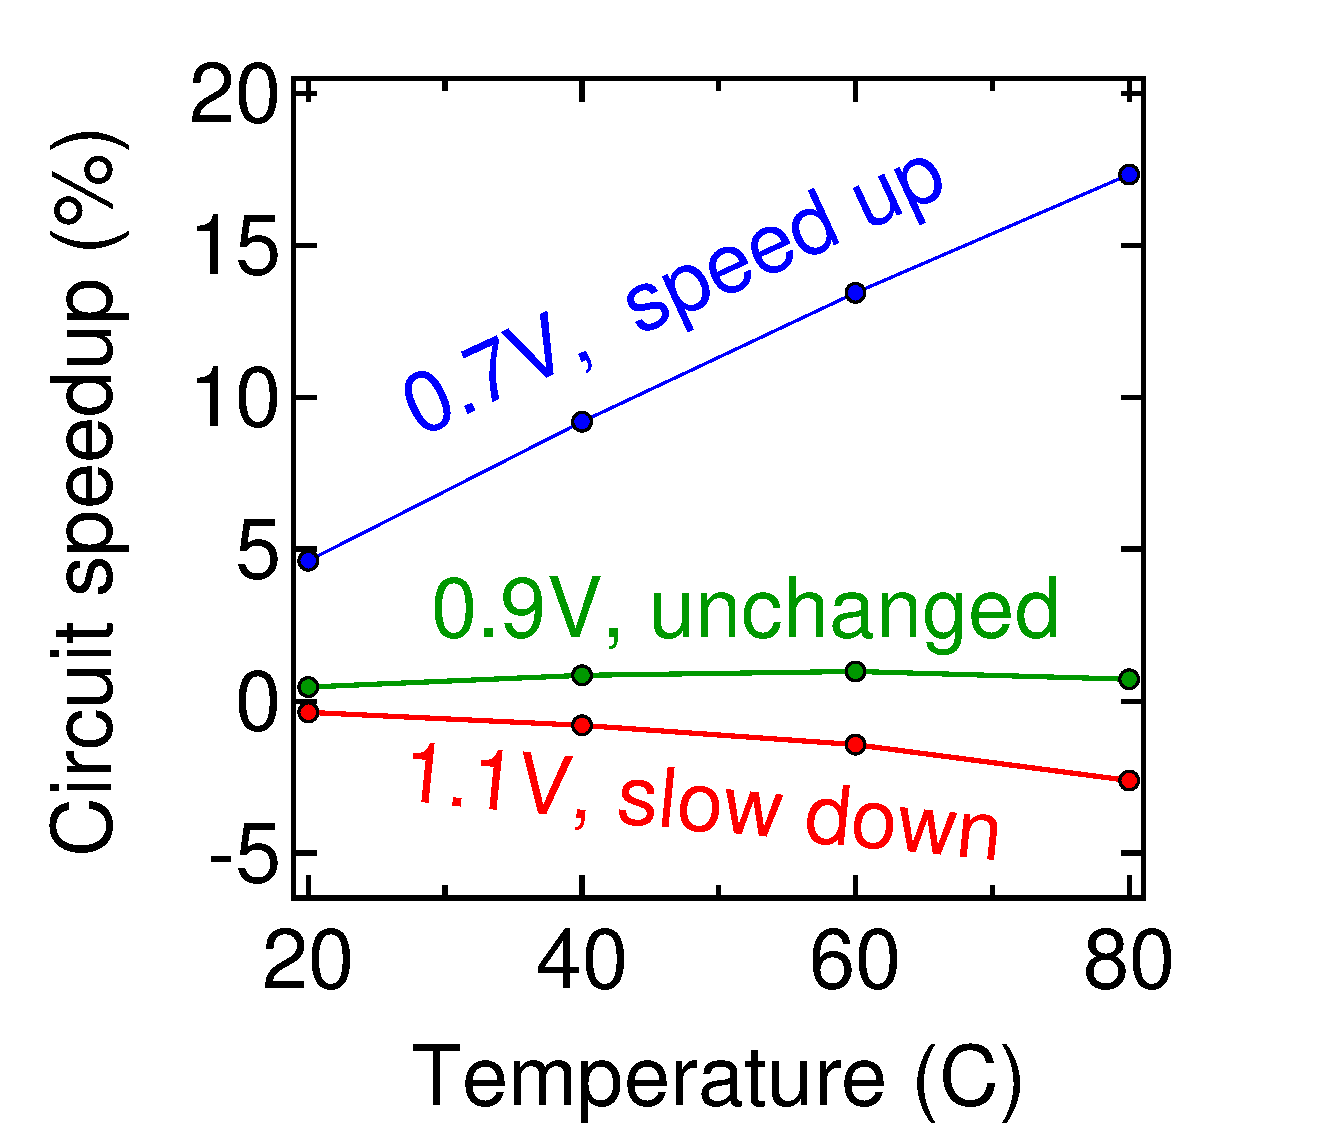
\includegraphics[trim=20 0 0 20,clip,width=0.35\linewidth]{graphs/temperature/motivation1.pdf}
  \label{fig:motivation1}
}
\hspace{0.4in}
\subfloat[Temperature inversion's inflection voltage approaches nominal supply.] 
{
  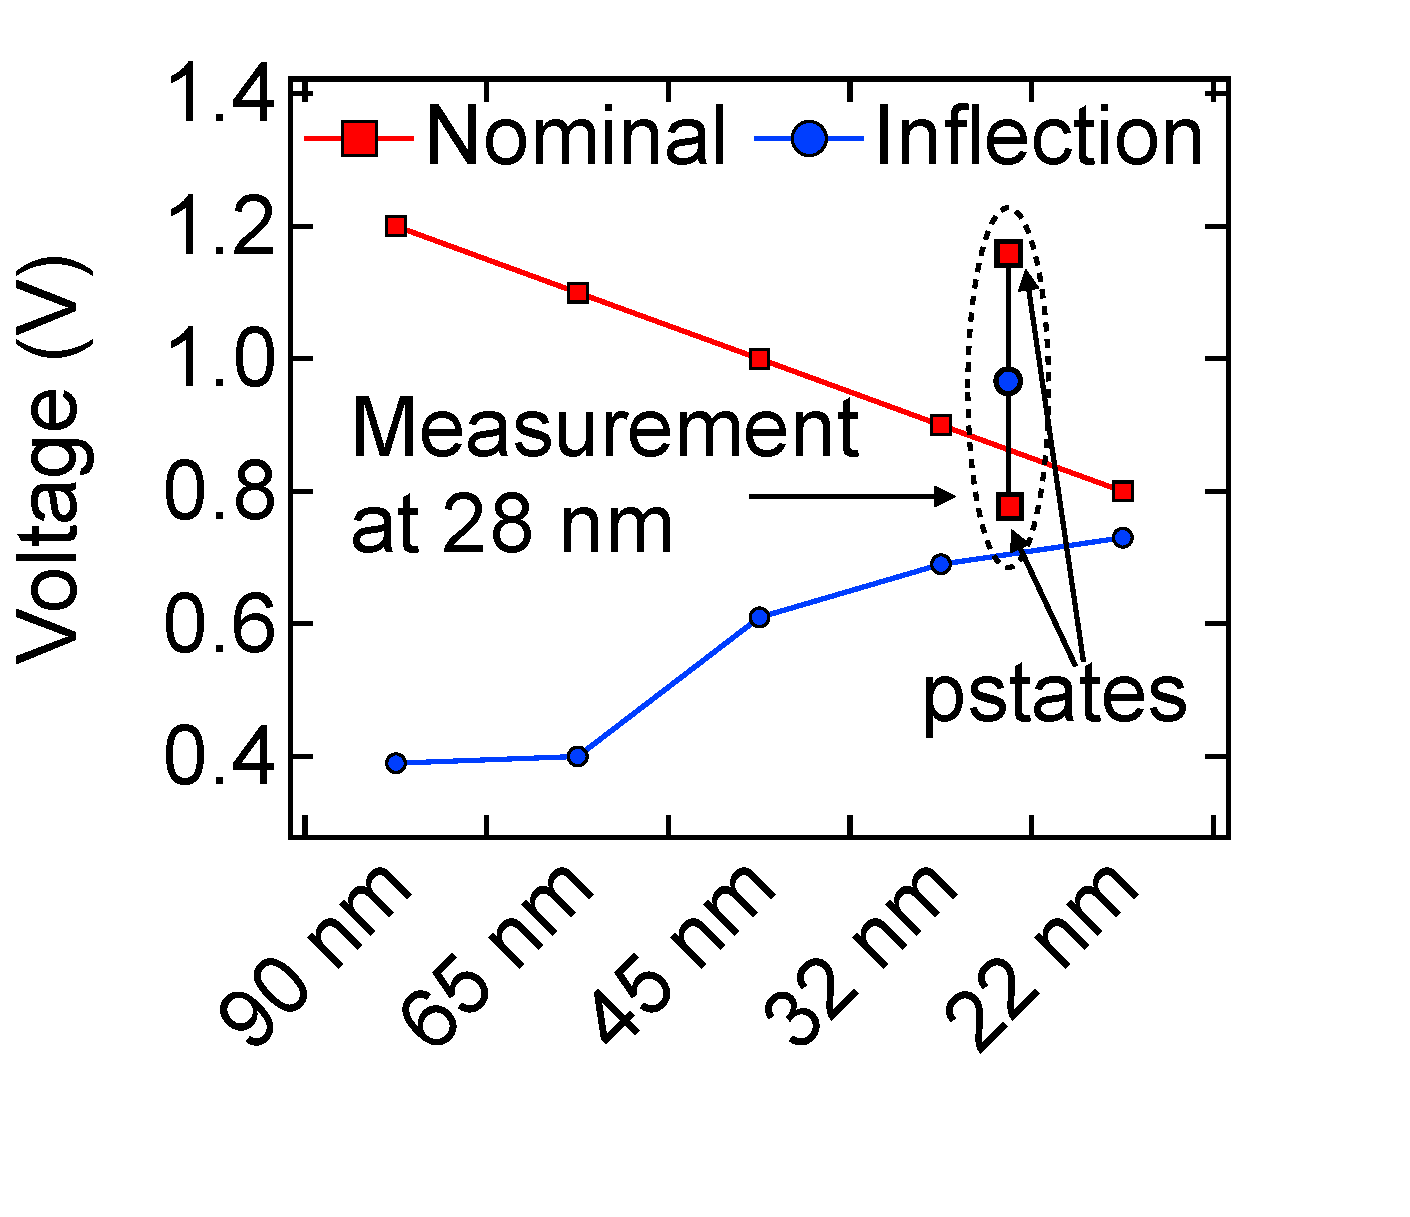
\includegraphics[trim=10 40 40 20,clip,width=0.35\linewidth]{graphs/temperature/motivation2.pdf}
  \label{fig:motivation2}
}
\caption{Temperature inversion is having more impact on processor performance as technology scales.}
\label{fig:motivation-plots}
\vspace{-0.2in}
\end{figure}

At a high level, the reason why temperature inversion occurs is a resulting of two fundamentally conflicting effects - when the temperature increases both carrier mobility and threshold voltage decrease. Carrier mobility decrease causes devices to slow down while threshold voltage reduction causes the devices to speedup. Temperature inversion happens in the region where the supply voltage is low enough to make the second factor (i.e., threshold voltage reduction) dominate, which is 0.7 V in~\Fig{fig:motivation1}. Otherwise, the devices slow down at the higher temperature, degrading performance as in the case of 1.1 V. 

In the past, temperature inversion has been safely discounted by processor designers because the nominal supply voltage at which this effect starts to occur is too low in prior technologies. At 250~nm, when temperature inversion was first discovered, the inflection voltage was more than 1.5~V lower than the nominal supply voltage~\cite{park1995reversal,bellaouar1998supply,dasdan2006handling}. With such a wide margin of separation, temperature inversion does not interfere with the processor's normal operating voltage region.

However, with technology scaling, today's processors are operating close to the temperature inversion's voltage region. Thus, the impact of this effect can no longer be safely discounted. \Fig{fig:motivation2} shows a detailed device analysis based on predictive technology models~\cite{wolpert2012temperature,zhao2006new}. As technology scales down from 90~nm to 22~nm, the inflection voltage increases with smaller feature sizes. At the 32~nm node, the inflection voltage is predicted to closer to the nominal supply voltage. Scaling into future FinFET and FD-SOI devices with smaller feature sizes, it is likely that temperature inversion will occur for all of a processor's operating voltage range~\cite{lee2014dynamic,cai2015tei}.

Silicon measurements performed on the AMD\textsuperscript{\textregistered} A10-8700P processor confirm this behavior in practice. At the 28~nm node, the inflection voltage in~\Fig{fig:motivation2} falls within the range of the processor's different P-states. The integrated GPU's highest P-state is only slightly above the inflection point. 

The fact that temperature inversion is the major temperature-related effect that varies circuit speed and timing margin today, and the fact that it has been neglected by the architecture community in the past make it imperative to thoroughly investigate the potential implications temperature inversion imposes on timing margin and architecture design. For this reason, we focus on exploiting temperature inversion for actively provisioning timing margin depending on runtime temperature level and transistor temperature inversion intensity. The rest of this section is organized as follows: \Sec{sec:temperature:setup} explains our experimental setup, \Sec{sec:temperature:characterize} systematically characterize how temperature affects circuit speed in contemporary microprocessors, \Sec{sec:temperature:tistate} proposes our \tistate solution for active timing margin, \Sec{sec:temperature:manage} discusses how to manage systems equipped with \tistates, and \Sec{sec:temperature:related} addresses related work.

\section{Experimental Setup}
\label{sec:temperature:setup}

In this subsection, we provide an overview of the experimental platform to study temperature inversion, including the chip under study and our temperature control mechanism. In particular, we explain the timing margin sensor we use, which serves as \textit{power supply monitor} in this chip. Timing margin sensor is the key element of our work.

\begin{figure}[t!]
  \centering
  \begin{minipage}{0.45\linewidth}
    \centering
                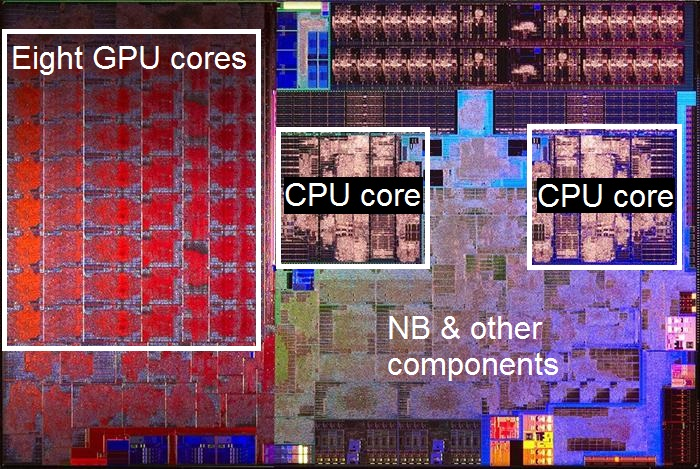
\includegraphics[trim=0 0 0 0,clip,height=1.5in]{graphs/temperature/carrizo-die.jpg}
                \caption{Die photo of the A10-8700P SoC.}
                \label{fig:die-shot}
  \end{minipage}
\hfill
  \begin{minipage}{0.45\linewidth}
    \centering
                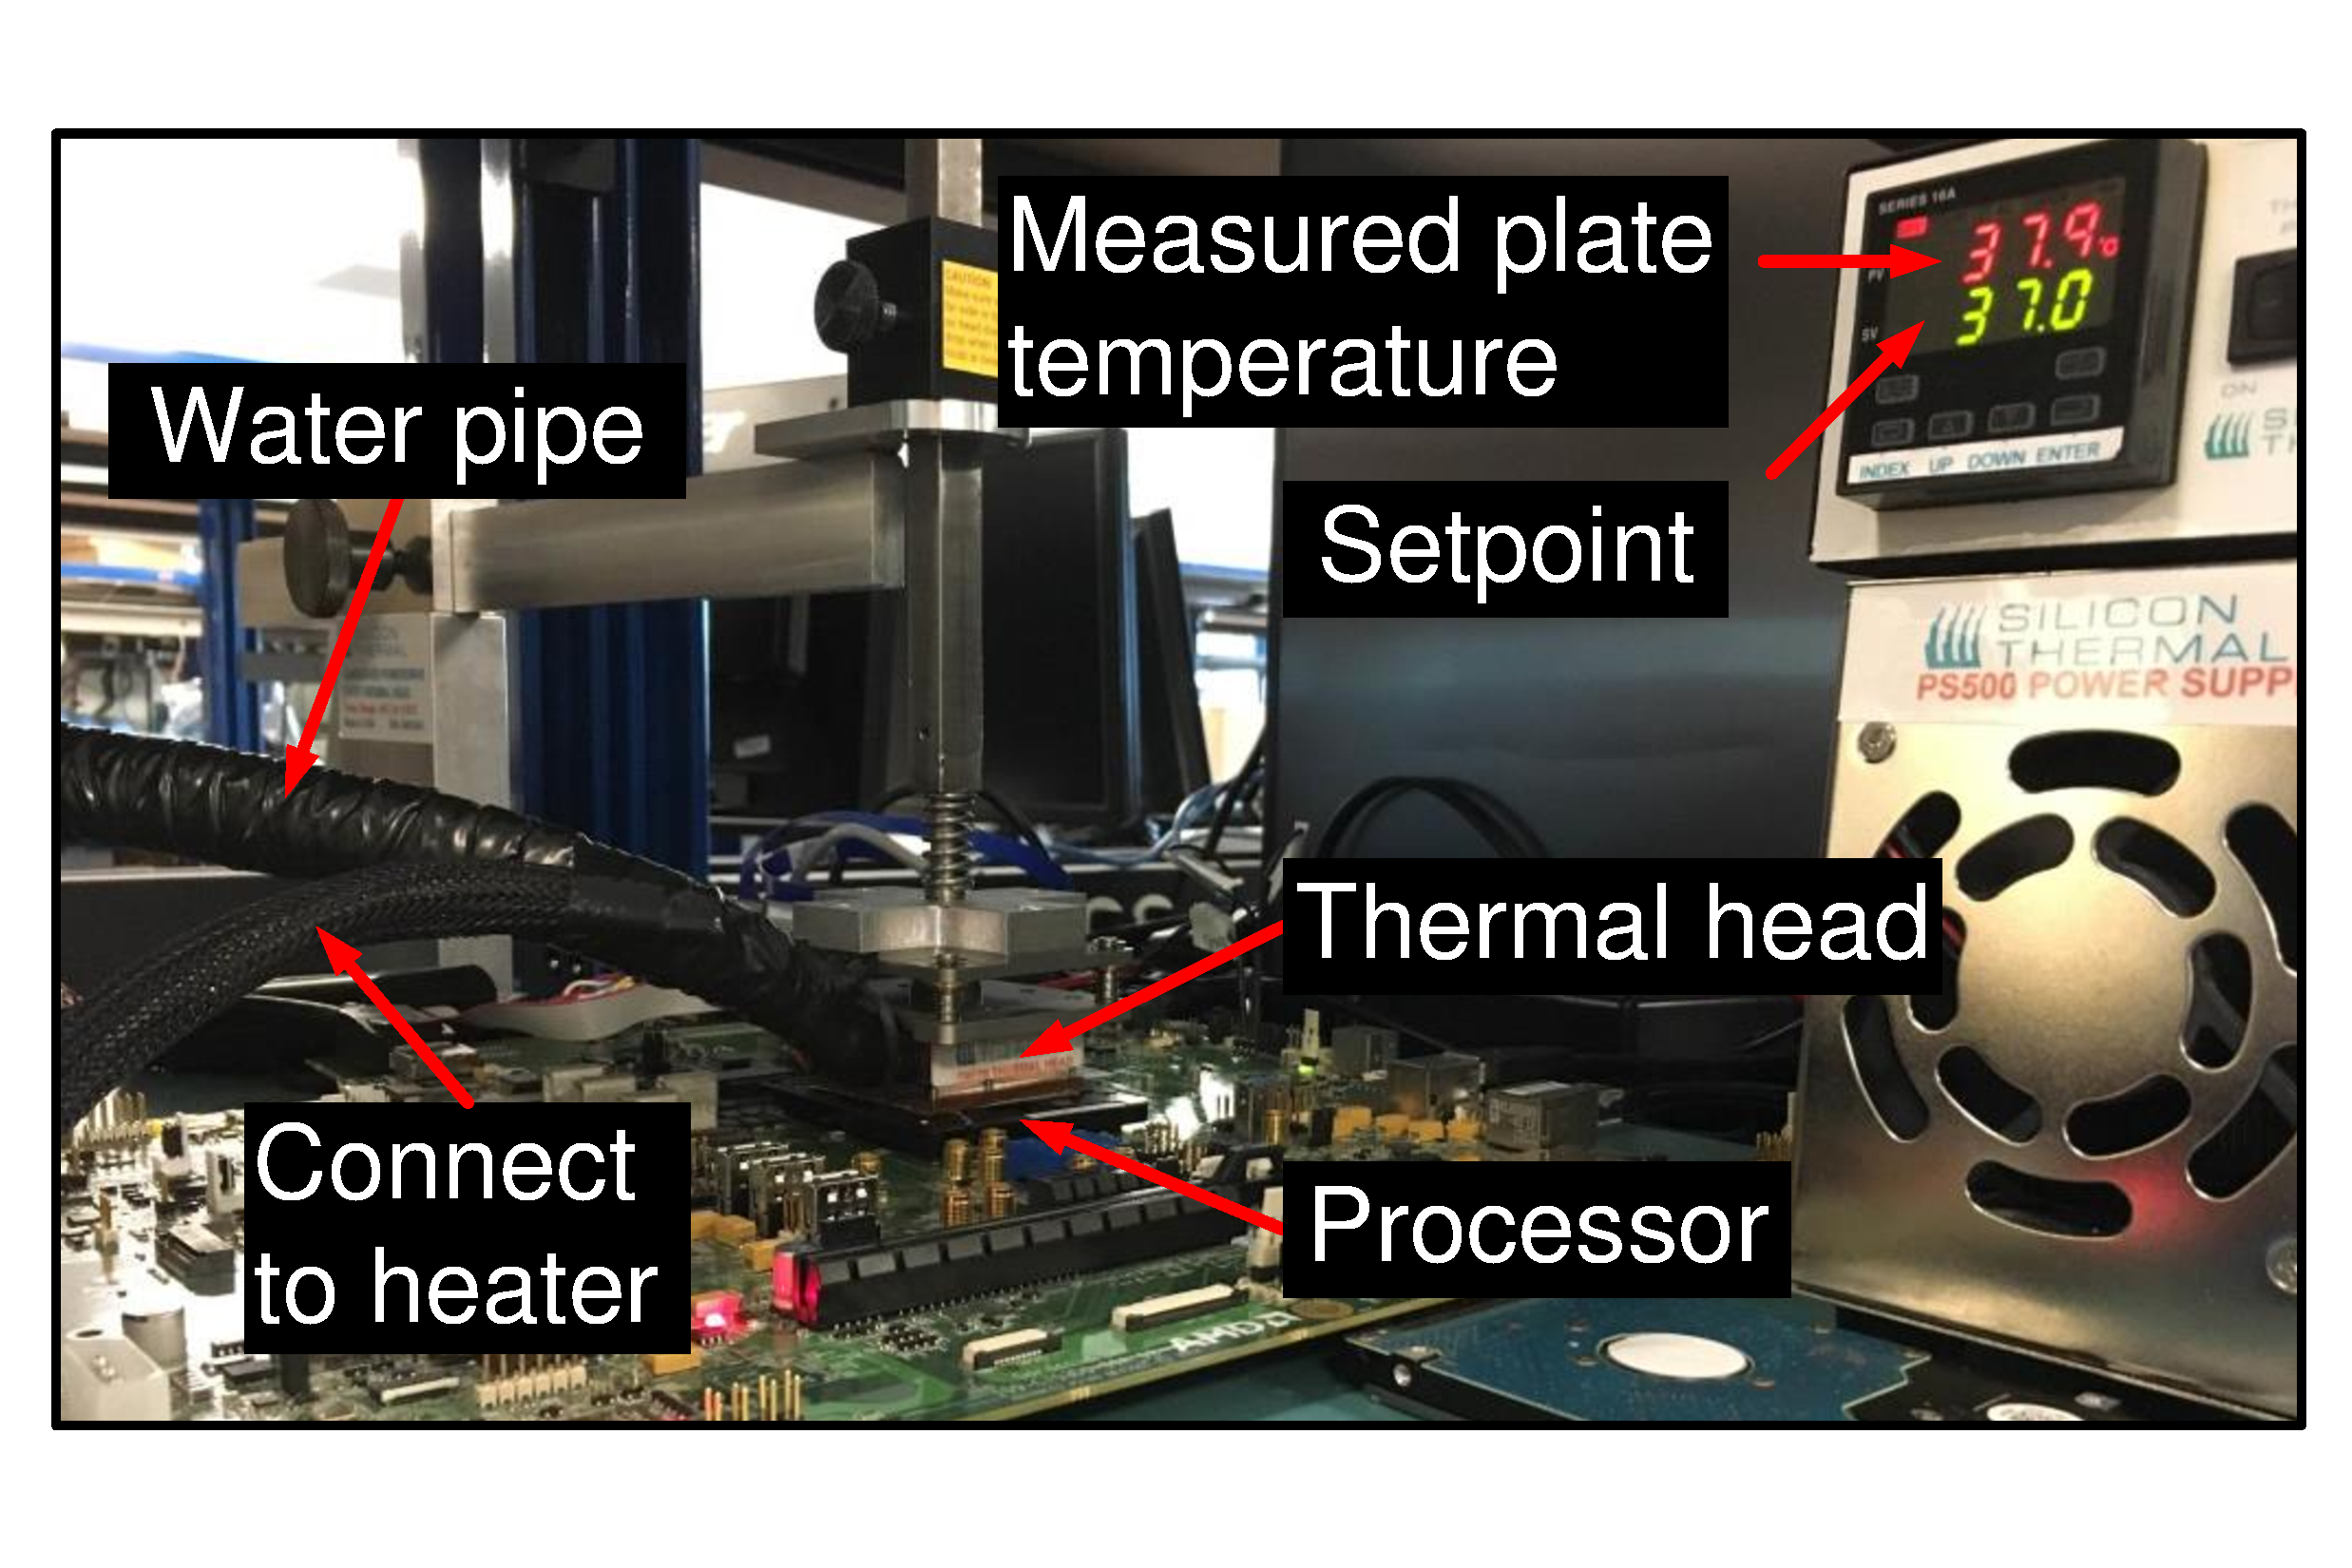
\includegraphics[trim=0 55 0 55,clip,height=1.5in]{graphs/temperature/temperature-control.pdf}
                \caption{Temperature control setup.}
                \label{fig:temp-control-photo}
  \end{minipage}

\end{figure}

\subsection{AMD\textsuperscript{\textregistered} A10-8700P Accelerated Processing Unit}
\label{sec:temperature:setup:apu}

The AMD\textsuperscript{\textregistered} A10-8700P Accelerated Processing Unit (APU) is an SoC manufactured in 28 nm HKMG planar bulk technology. It integrates two CPU core-pairs, eight GPU cores, and other components as shown in~\Fig{fig:die-shot}. Each CPU core-pair contains two out-of-order cores that share the front-end and floating point units. Each GPU core includes four 16-lane wide single instruction multiple data (SIMD) units. 

We conducted temperature inversion studies on both the CPU and GPU. A separate power delivery network allows us to control the CPU and GPU voltage independently. But in this work, we present the results for the GPU only because the GPU's throughput-oriented architecture allows low-voltage region operation with meaningful and realistic performance. However, because the temperature inversion effect we study depends solely on the supply voltage, and not necessarily the underlying architecture, the analysis and benefits we present on the GPU naturally do extend to the CPU as well.

The GPU clock is set at 300 MHz in the voltage region we explore around 0.7~V. We pick 300MHz because its associated low voltage is within the temperature inversion region, and makes it possible to explore the potential impact of temperature inversion on future near-threshold technologies. The 300 MHz frequency corresponds to the GPU's lowest P-State, and in practice we have observed this P-State being exercised frequently during normal workload execution. 

We use the ATITool~\cite{atitool} to set the GPU's voltage and frequency over a wide operating range. To measure power, we use a National Instrument's DAQ that reads the GPU's isolated supply voltage rail once every 10~ms.

\subsection{Temperature Control Setup}
\label{sec:temperature:setup:temp}

To characterize temperature inversion's effect on performance and power under different operating conditions, we have to carefully regulate the processor's on-die temperature. In our work, we generally sweep temperature range from 0\C to 80\C. This temperature range falls within the product's operating temperature range, and does not affect aging significantly.

\Fig{fig:temp-control-photo} shows our temperature control setup. A thermal head is attached to the processor package. To stabilize the die temperature, which is measured via an on-chip thermal diode, at a user-specified target value, the thermal head's temperature is adjusted every 10~ms. Physically, the thermal head's temperature is controlled via a water pipe and a heater. The water pipe is connected to an external chiller to offer low temperatures while the heater increases temperature to reach the desired temperature setting. Under feedback control, we see a 2\C temperature variation on the diode in the worst-case. So, for instance, \Fig{fig:temp-control-photo} shows the thermal head set its temperature to 37\C to let the die temperature stay at 40\C. 

\subsection{Timing Margin Sensors: On-chip Power Supply Monitors (PSMs)}
\label{sec:temperature:setup:psm}

We use power supply monitors (PSMs)~\cite{grenat20145,gillespie2014streamroller} to accurately measure circuit speed changes in the chip under different temperature conditions. A PSM is a time-to-digital converter that reflects circuit time-delay or speed in numeric form. Originally designed as a voltage noise sensor, a PSM can sense minute circuit timing changes due to $di/dt$ droops~\cite{grenat20145}. We use the PSM as a means to characterize circuit performance under temperature variation.

\begin{figure}[h]
    \centering
    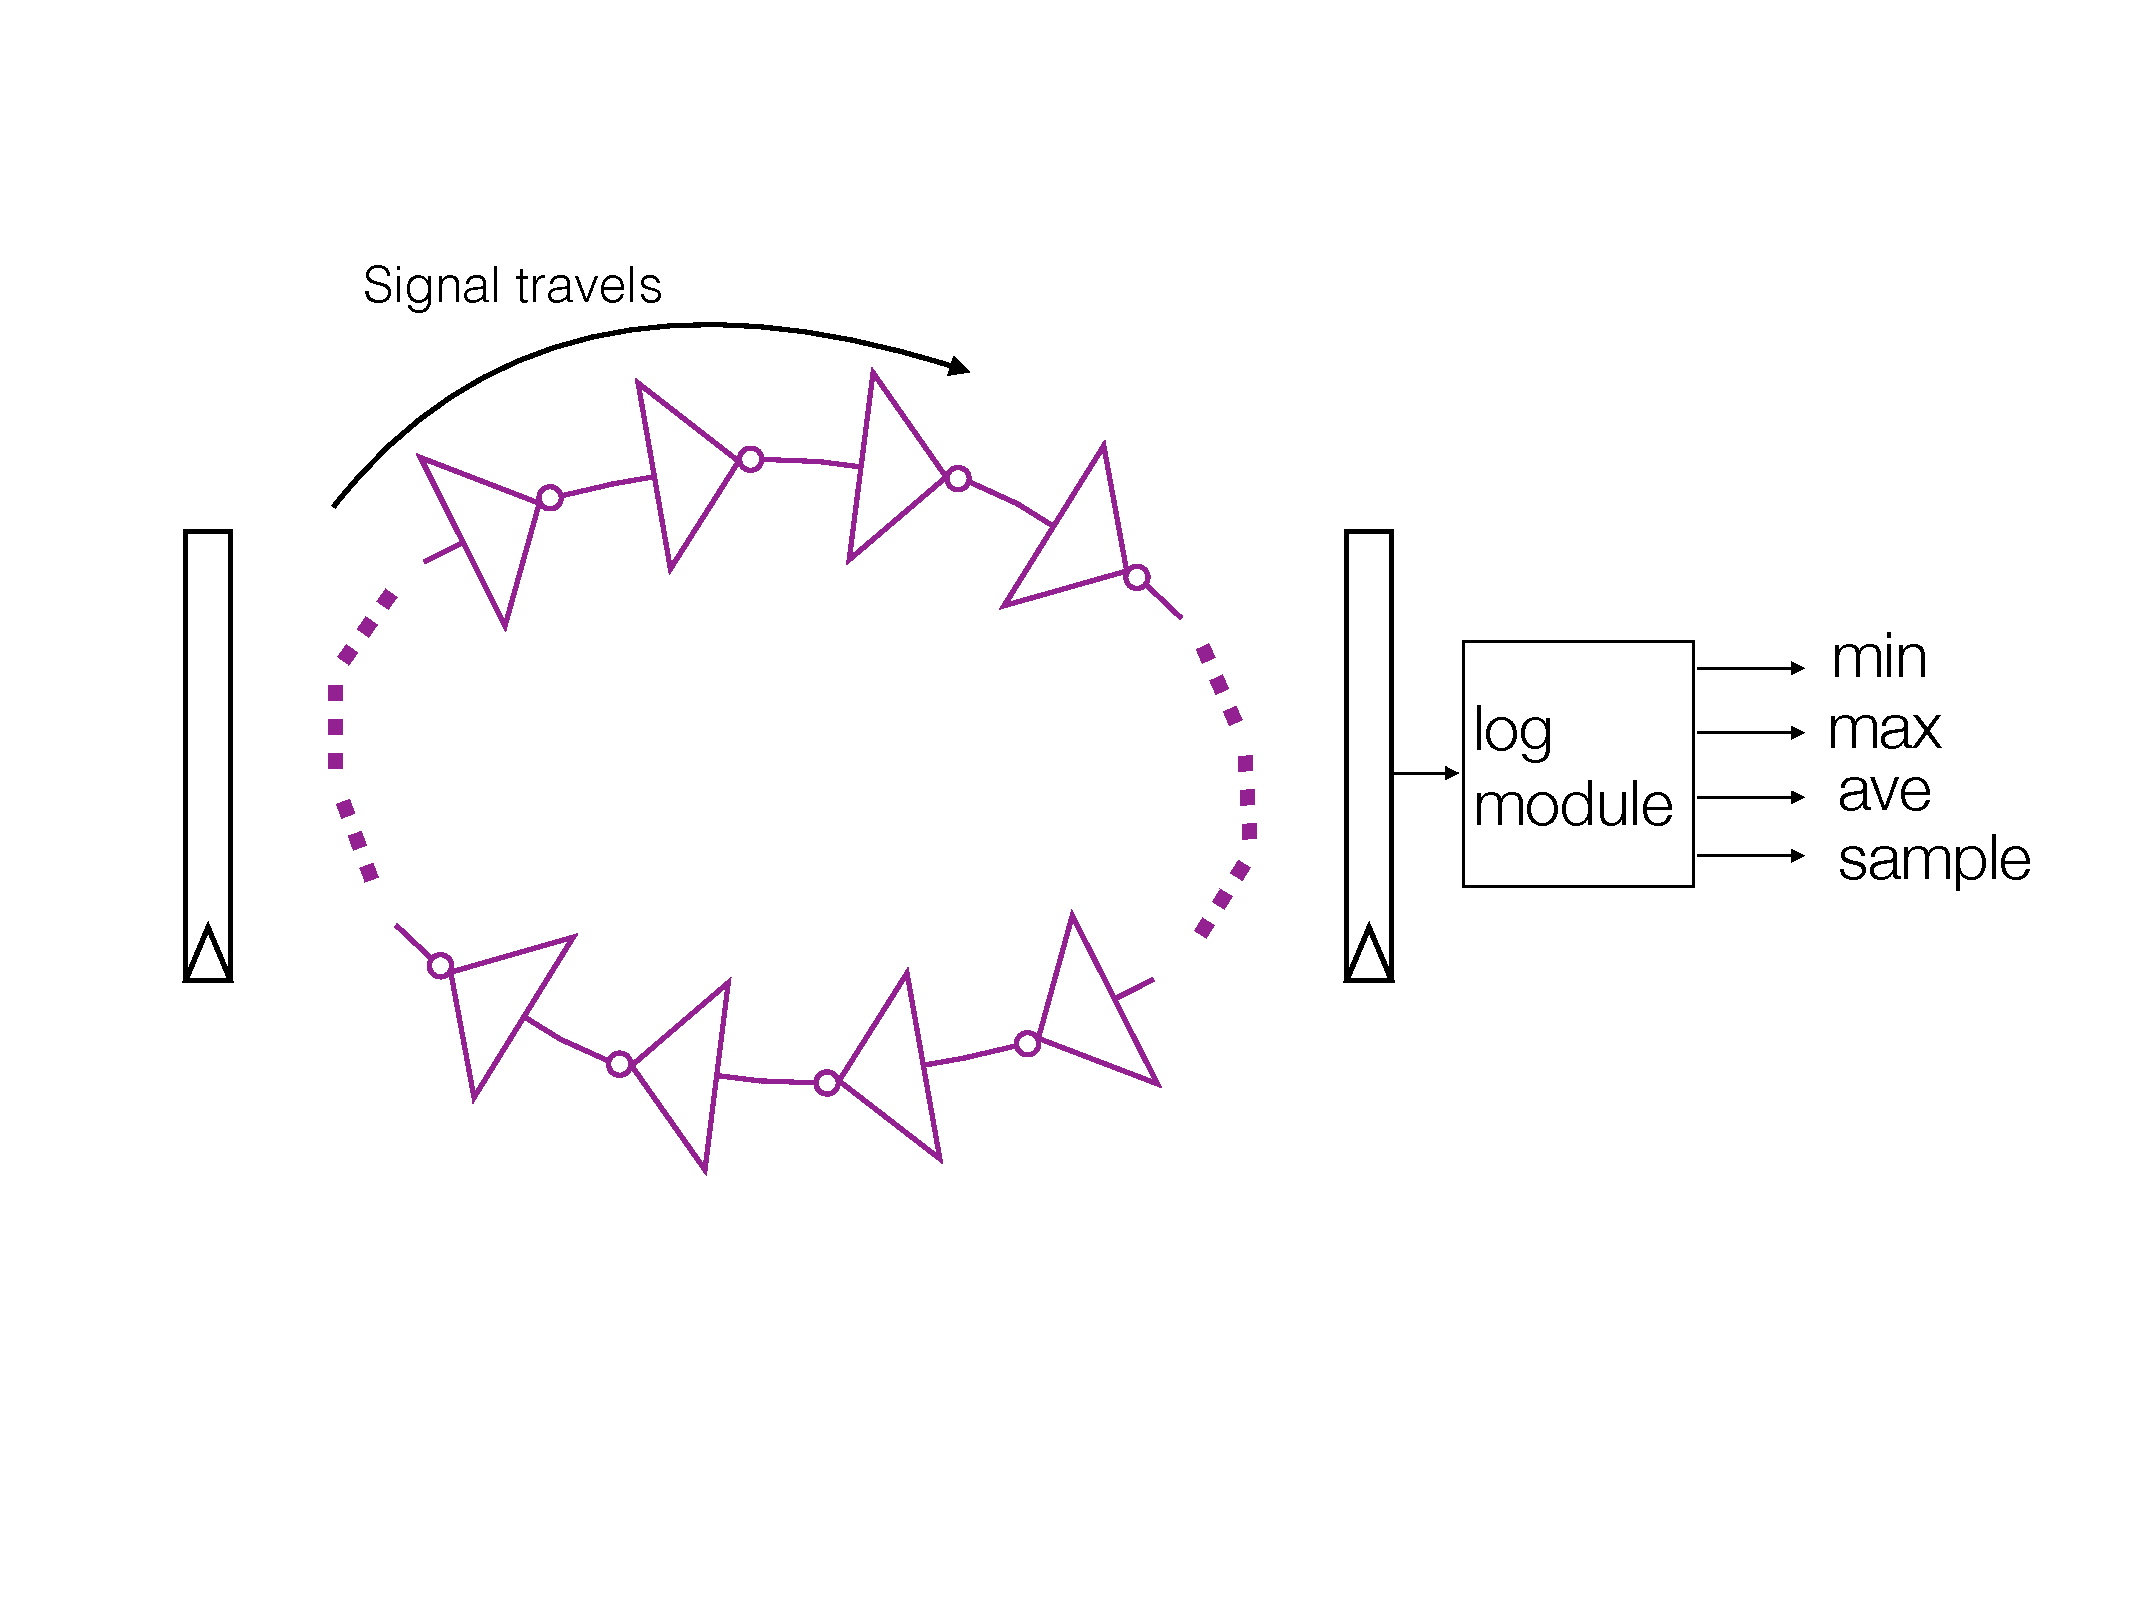
\includegraphics[trim=40 150 40 150,clip,width=0.8\columnwidth]{graphs/temperature/psm.pdf}
    \caption{Power supply monitors (PSMs) measures pipeline speed/timing margin with an inverter ring. By counting how many inverters an edge has traveled through, the PSM reports a digital value that reflects circuit speed.}
    \label{fig:psm-struct}
\end{figure}

\Fig{fig:psm-struct} shows the structure of a PSM. Its core component is a ring oscillator that counts the number of inverters an ``edge'' has traveled through in each clock cycle. When the circuit is faster (e.g., under smaller $di/dt$ effects or stronger temperature inversion), an edge can pass more inverters and PSM will produce a higher count output. A supporting module logs ring oscillator's per-cycle output and accumulates the minimum, maximum, and average values over a time.

The A10-8700P processor has ten PSMs in each CPU core-pair and two PSMs in each GPU core, distributed across the cores to account for process variation and spatial differences in $di/dt$ effect. Through measurements we determined that the changes in the different PSM readings under different temperatures are nearly identical, thus we only show the result of one representative PSM in GPU. The results are representative of using other or more than one PSM. 

For reasons that prevent us from showing absolute values, we normalize the PSM reading to a reference value measured under 0.7~V, 300~MHz, 0\C, and idle chip condition. We log the minimum, maximum, and average output of all the PSMs. 

\section{Characterizing Timing Margin Under Temperature Inversion Variation}
\label{sec:temperature:characterize}

In this section, we first view the timing margin sensor (i.e., PSM) as a normal logic path to understand circuit performance under different temperature environment (\Sec{sec:temperature:characterize:psm}). Then, we use the circuit speed difference to extrapolate how much extra margin can be squeezed out due to timing margin change caused by temperature inversion variation (\Sec{sec:temperature:characterize:extrapolate}).

\subsection{Circuit Speed Variation Under Different Temperature}
\label{sec:temperature:characterize:psm}

The PSM by itself is a digital circuit located between the pipeline latches with other normal logic paths~\cite{sriram2016avfs}, and therefore its speed characteristics are representative of a pipeline's overall performance. For this reason, we use the PSM's output to quantify circuit performance across a wide range of different steady-state temperatures. 

\begin{figure}
\centering
    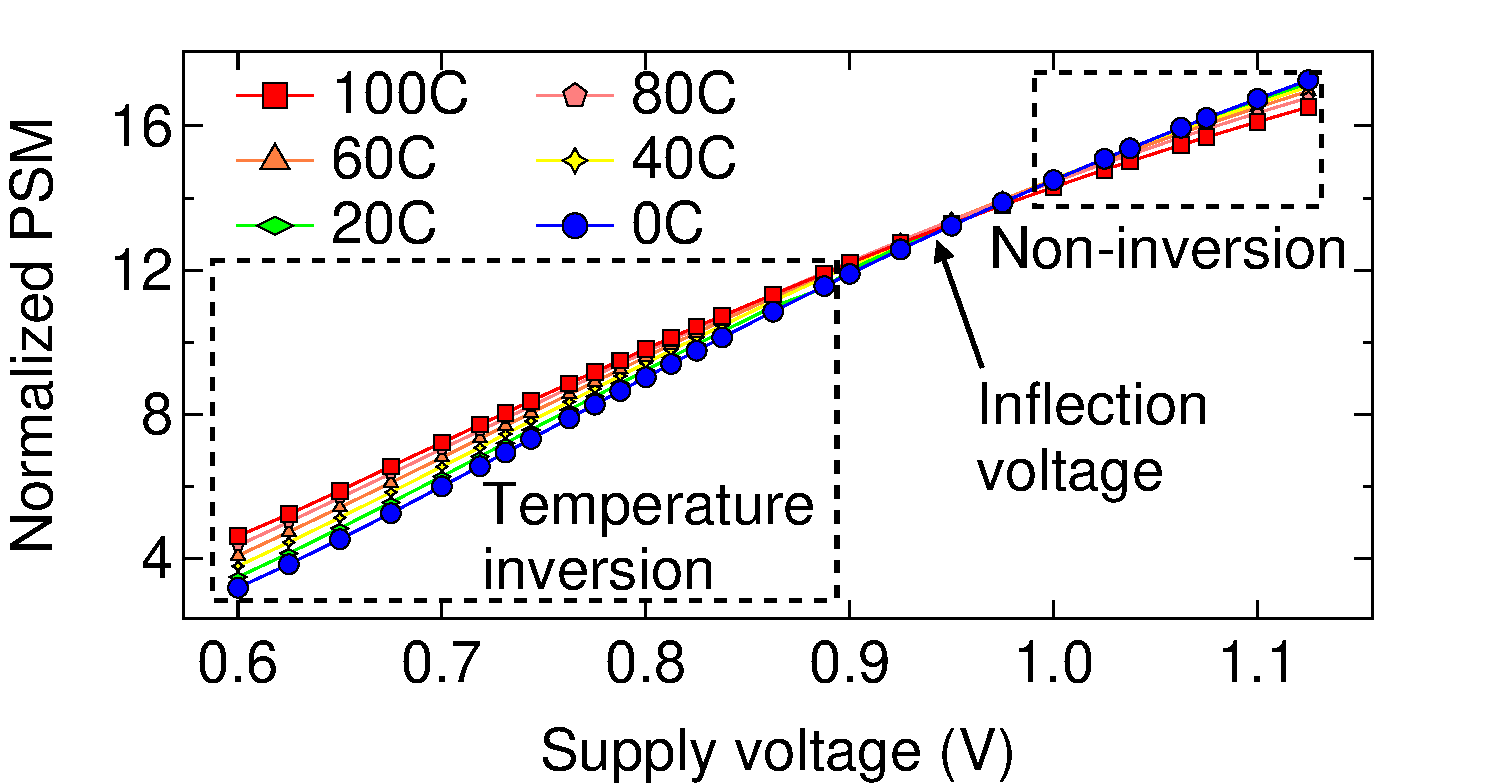
\includegraphics[trim=0 0 50 20,clip,width=.9\linewidth]{graphs/temperature/idle-psm-volt-temp.pdf}
    \caption{Temperature inversion happens below 0.9~V and is progressively stronger when voltage scales down.}
    \label{fig:psm-wide-range}
\end{figure}

We keep the chip idle (i.e., the clock is still running) and read the PSM's ``average'' value to exclude the $di/dt$ effect caused by workload dynamics. \Fig{fig:psm-wide-range} shows the circuit speed under different supply voltages and die temperatures. Speed is reflected by the PSM's normalized output -- higher value implies a faster circuit. At a higher supply voltage, the circuit switches faster, and the PSM can travel more inverters in a cycle which produces a higher count. The voltage-to-PSM relationship conforms to similar analysis as in~\cite{zu2015adaptive}.

We find that temperature's impact on circuit performance depends on the supply voltage. In the high supply voltage region around 1.1 V, the PSM's reading becomes progressively smaller as the temperature rises from 0\C to 100\C. The circuit is operating slower at a higher temperature, which aligns with conventional belief~\cite{leng2015safe}. The reason for this circuit performance degradation is that the transistor's carrier mobility decreases at a higher temperature, leading to smaller switch-on current ($I_{on}$) and longer switch time~\cite{wolpert2012temperature}.

Under a lower supply voltage, the PSM's reading increase with higher temperature, which means the circuit switches faster (i.e., the temperature inversion phenomenon). During temperature inversion the transistor's threshold voltage ($V_{th}$) decreases linearly as temperature increases~\cite{wolpert2012temperature,park1995reversal,dasdan2006handling}. Thus, for the same supply voltage, a lower $V_{th}$ provides more drive current ($I_{on}$) which makes the circuit switch faster. The speedup effect is more dominant when supply voltage is low because then the supply voltage is closer to $V_{th}$.

When the supply voltage is low enough, the speedup contribution from the reduced $V_{th}$, at some point, will balance out the carrier mobility slowdown. We call this voltage point the {\it inflection voltage}. The inflection voltage may change from chip to chip due to $V_{th}$ variations, and it can be characterized during the binning process. In~\Fig{fig:psm-wide-range}, we show that the tested processor's inflection voltage is between 0.9~V and 1~V. In this region, the temperature does not have a notable impact on circuit performance. Below the inflection voltage (0.95~V) is the temperature inversion region while above it is the non-inversion region. Half of the GPU's P-states, which range from 0.75~V to 1.1~V, operate in the temperature inversion region.

In~\Fig{fig:psm-wide-range}'s temperature inversion region, the speed change between any two temperatures increases when the supply voltage scales further away from the inflection point. As voltage scales into the lower voltage region around 0.6~V, the PSM reading varies by more than 40\%, indicating the drastic speedup at a higher temperature. As voltage goes lower towards the near-threshold region, the overdrive voltage ($V_{dd}-V_{th}$) becomes small and it is very sensitive to small $V_{th}$ changes. Thus, temperature inversion's $V_{th}$ reduction has a more significant impact on device performance.

\begin{figure}
    \centering
    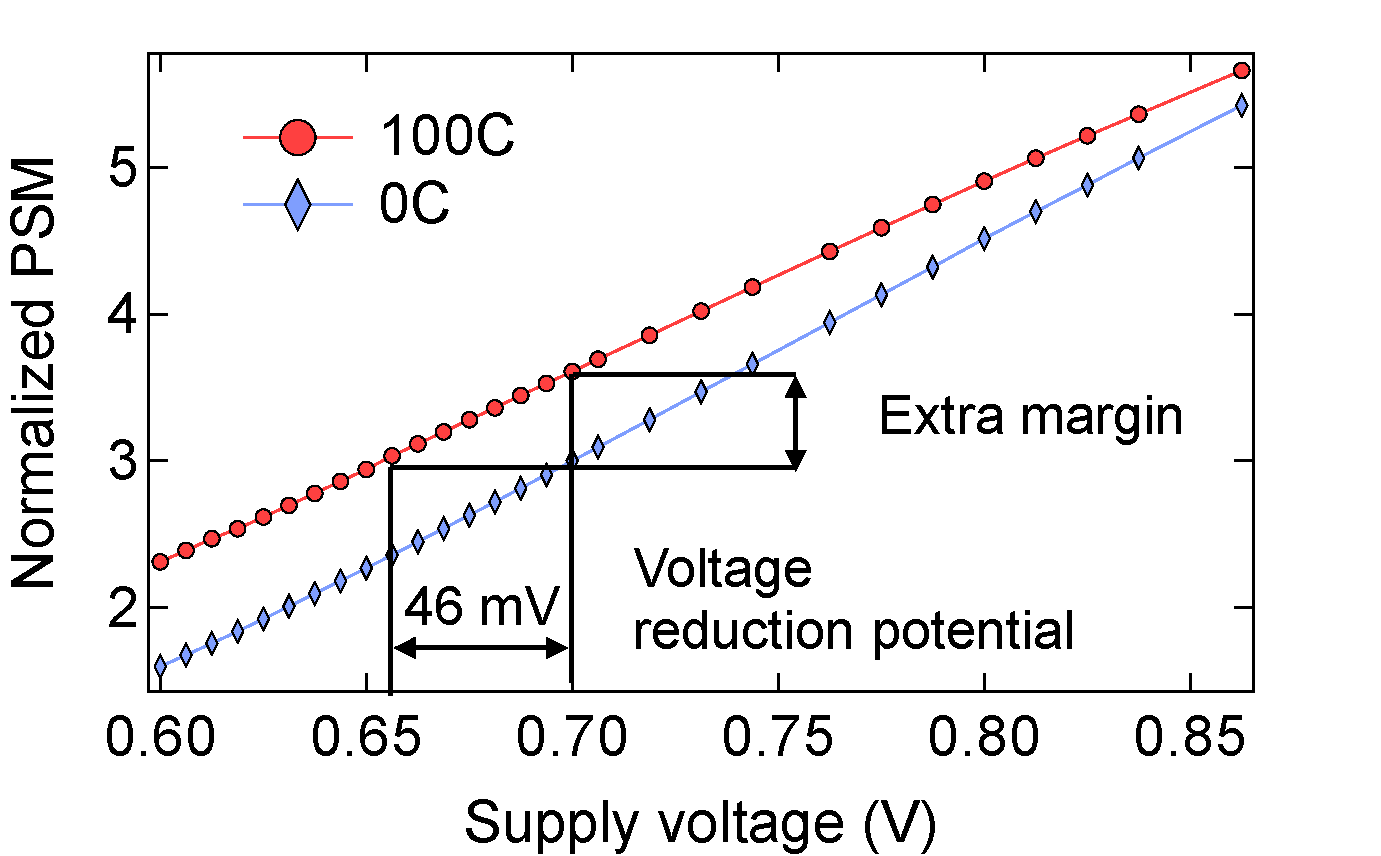
\includegraphics[trim=0 0 50 20,clip,width=.8\linewidth]{graphs/temperature/idle-psm-volt-nt.pdf}
    \caption{Estimating voltage reduction potential based on PSM characterization at different temperatures.}
    \label{fig:psm-nt}  
\end{figure}

\Fig{fig:psm-nt} zooms into the low voltage region between 0.6~V and 0.86~V and has a clearer view of temperature inversion. The figure shows temperature inversion's performance benefit at 100\C over the 0\C baseline, and this benefit increases as the supply voltage decreases. Hereon forward we use temperature inversion at 0.7~V as a case study to dive deeper and get more insights. Although we restrict ourselves to this single voltage, there is ample opportunity to demonstrate how temperature inversion may add new ingredients to overall system management.

\subsection{Estimating Active Timing Margin's Undervolting Opportunity}
\label{sec:temperature:characterize:extrapolate}

In this subsection, we provide a ``design space exploration'' of active timing margin's voltage reduction opportunity. When running workloads, chip temperature frequently goes up and speeds up circuits because of temperature inversion. This adds extra timing margin in the pipeline, and the extra margin can be exploited via undervolting. 

To determine the amount of extra timing margin that can be exploited, we first need a ``baseline margin'' where timing margin is not overprovisioned for temperature variation. In other words, the ``baseline margin'' is the timing margin allocated for the worst-case temperature. It can tolerate all other effects such as $di/dt$ and aging at worst-case temperature, yet circuit speed can not be degraded anymore compared to worst-case temperature. When undervolting, it is crucial that the system only reclaims the extra timing margin added from this ``baseline margin'' and does not reclaims anymore. Otherwise, pipeline timing may fail under some worst-case workloads, such as in the case of voltage stressmarks~\cite{kim2012audit,bertran2014voltage}. 

We use the timing margin measured at 0\C as the ``golden'' reference when reclaiming temperature inversion's extra margin. In other words, the timing margin delivered by our active timing margin scheme should match the ``golden'' reference. Under this constraint, we can undervolt to maximize power saving. 

We choose 0\C as the reference because under temperature inversion lower temperature degrades circuit performance. Even though 0\C rarely occurs in desktop, mobile, and datacenter applications, the timing margin still needs to be set to tolerate this worst-case condition. In the industry, 0\C or below is used as a standard circuit design guideline~\cite{altera2010timing}. In certain scenarios, such as military use, an even more conservative reference of -25\C is considered~\cite{dasdan2006handling}.

\Fig{fig:psm-nt} shows our estimation process of how much voltage can be reduced via active timing margin. The PSM difference between the high-temperature 100\C line and the ``golden reference'' line at 0\C represents the extra timing margin in the units of inverter delays. In other words, it reflects how much faster the circuits can run at a higher temperature. To bring the faster circuit back to the original speed, supply voltage needs to reduce such that under a higher temperature the PSM will ideally read the same value.

\begin{figure}
  \centering
  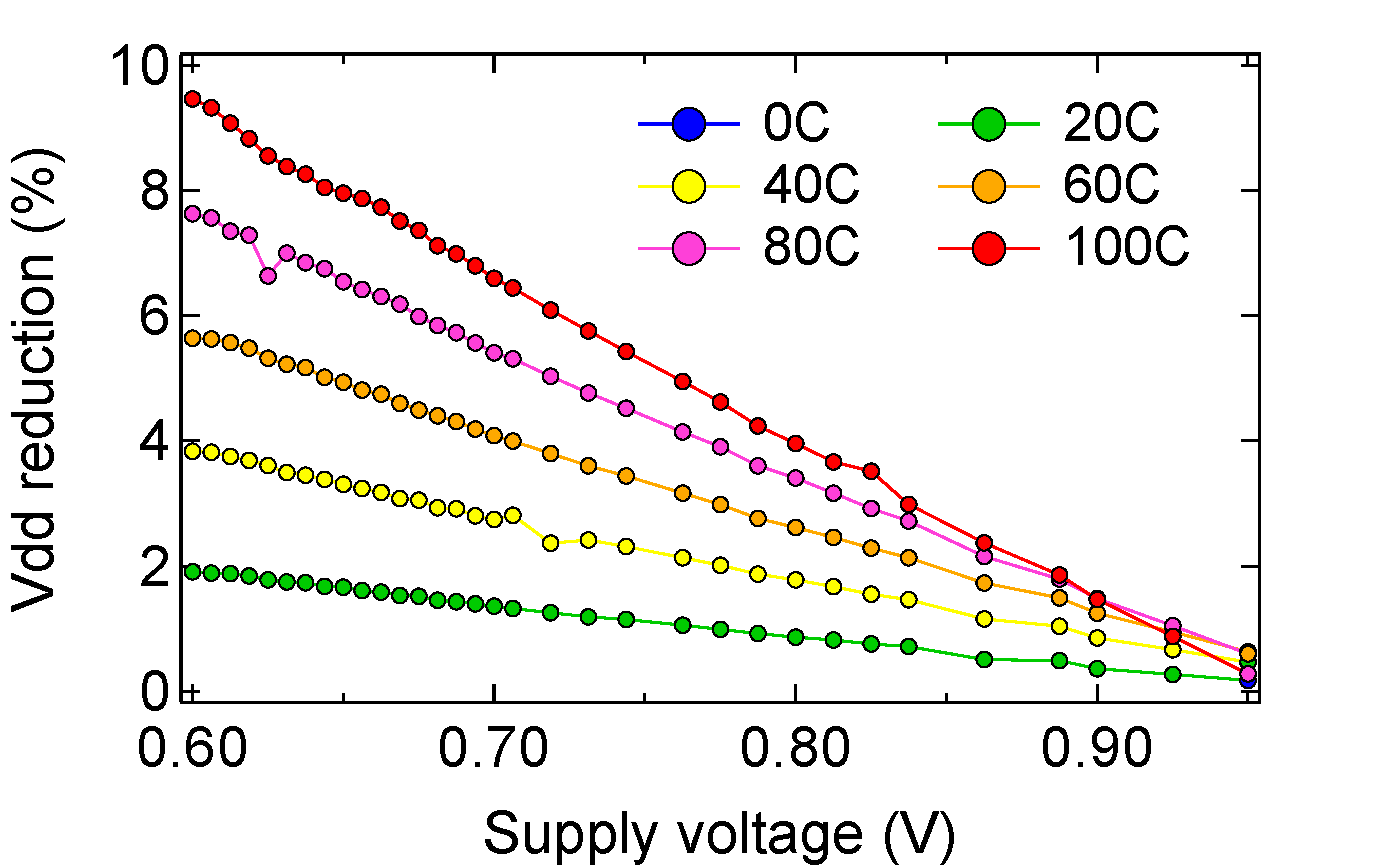
\includegraphics[trim=0 0 50 20,clip,width=.8\linewidth]{graphs/temperature/extrapolate-uv-potential.pdf}
  \caption{Voltage reduction potential is more pronounced in the near-threshold low voltage region.}
  \label{fig:uv-potential} 
\end{figure}

We estimate the voltage reduction potential with linear extrapolation.~\Fig{fig:uv-potential} shows the estimated opportunity at different temperatures. As supply voltage scales down, the voltage reduction potential goes up almost linearly. Temperature inversion effect is stronger in the lower voltage regions, and hence the greater timing margin opportunity. At 0.6~V and 100\C, the extra timing margin provided by temperature inversion can turn into almost 10\% voltage reduction compared to 0\C. As a reference, 5\% voltage reduction is considered significant in previous works~\cite{webel2015robust}. At 0.7~V in our study, we can have 1.5\% to 7\% voltage reduction potential depending on the processor temperature.


\section{Temperature Inversion States (Ti-States)}
\label{sec:temperature:tistate}

Having understood temperature inversion's potential for active timing margin, we propose a systematic method to establish a precise and reliable temperature to voltage mapping that implements active timing margin. The temperature to voltage mapping is discrete as voltage regulator module's output voltage is quantized in small steps~\cite{intelVRM}. The final mapping is, therefore, in a table format, which we call \tistates. Similar to the way P-states functions for DVFS, \tistate is a natural evolution of power management mechanisms for active timing margin.

\subsection{Methodology to Construct the Ti-States Table}
\label{sec:temperature:temperature:construct}

We propose a workload-centric methodology that constructs a set of temperature-voltage states in the inversion region (\tistates) at test-time. A workload-centric approach ensures \tistates will work in the face of workload-induced uncertainties like $di/dt$ and IR effects. We use a subset of workloads as the ``training'' set to first get a tentative temperature-voltage mapping. Then we validate this mapping with another set of ``test'' workloads to establish the final \tistate. During training the \tistate is constructed in a manner that is agnostic to workload-specific settings, so we can be sure our voltage selection will provide enough margin for any workload that is run on the processor.

For each of the training workloads, we first measure their ``golden'' reference margin at 0\C. Then, at the temperature being characterized, we select four candidate voltages. These candidates voltage are picked such that they are around the extrapolated voltage value from~\Fig{fig:uv-potential}. The candidates voltages are chosen such that they are two VRM steps above and two VRM steps below the extrapolated value. 

\begin{algorithm}[h]
\caption{\tistate Construction Methodology}
\label{train-algo}
\begin{algorithmic}[1]
\Procedure{Get Reference Margin}{}
\State $\text{set voltage and temperature to reference}$ 

\For{each training workload} 
\State $\textit{workloadMargin} \gets \text{PSM measurement}$
\State $\text{push } \textit{RefMarginArr}\text{, }\textit{workloadMargin}$ 
\EndFor
\Return \textit{RefMarginArr}
\EndProcedure

\Procedure{Explore Undervolt}{}
\State $\textit{initVdd} \gets \text{idle PSM extrapolation}$ 
\State $\textit{candidateVddArr} \gets \text{voltage around }\textit{initVdd}$
\State $\textit{minErr} \gets \text{MaxInt}$ 
\State $\text{set exploration temperature}$

\For{each \textit{Vdd} in \textit{candidateVddArr}} 
\State $\text{set voltage to } \textit{Vdd}$

\For{each training workload} 
\State $\textit{workloadMargin} \gets \text{PSM measurement}$
\State $\text{push } \textit{TrainMarginArr}\text{, }\textit{workloadMargin}$ 
\EndFor

\State $\textit{err} \gets \text{diff(}\textit{RefMarginArr}\text{,}\textit{TrainMarginArr}\text{)}$
\If {$\textit{err} < \textit{minErr}$} 
\State $\textit{minErr} \gets \textit{err}$
\State $\textit{exploreVdd} \gets \textit{Vdd}$
\EndIf
\EndFor
\Return \textit{exploreVdd}
\EndProcedure

\end{algorithmic}
\end{algorithm}

Once we have the set of candidate voltages, we step through each candidate voltage and record the training workloads' timing margin using the PSM at every temperature that is being characterized. The timing margin measured at the candidate voltage is compared against the reference margin. Finally, we select the candidate voltage that has the minimum PSM difference from the golden reference. 

It is worthwhile to note that on our particular chip the data variation for the 16 PSMs on our GPU is under 2\%, so it makes little difference to use worst-case versus average. However, under severe intra-chip variation, transistor's undervolting potential can differ significantly. In that case, worst-case PSMs values need to be used for comparison.

\begin{figure}[t]
    \centering
    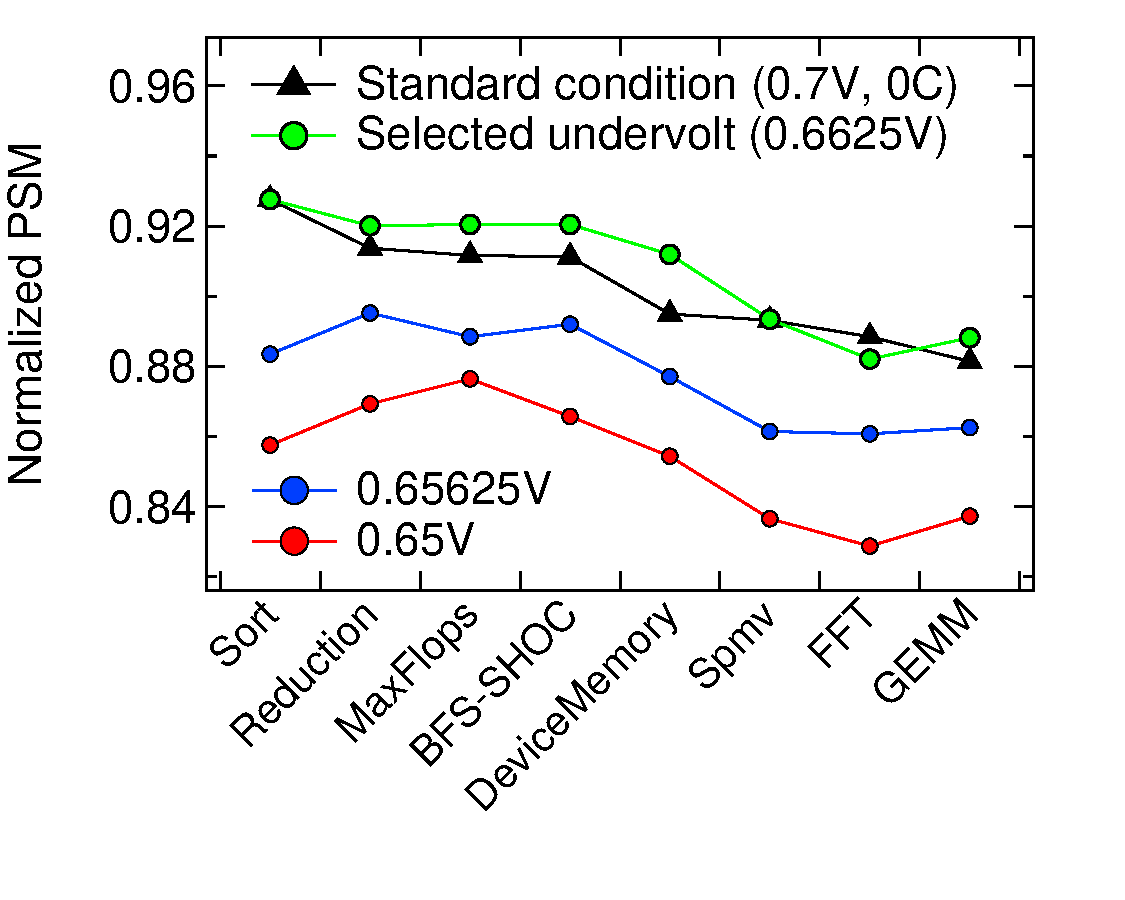
\includegraphics[trim=-30 0 0 0,clip, width=0.7\linewidth]{graphs/temperature/explore-uv-shoc.pdf}
    \caption{Exploring \tistate at 80\C: we measure the ``training'' workloads' timing margin, and choose the $V_{dd}$ that best tracks the standard margin.}
    \label{fig:train-uv}
\end{figure}

\Algo{train-algo} summarizes our methodology. \Fig{fig:train-uv} shows an example at 80\C. At this temperature, \Fig{fig:uv-potential}'s extrapolated voltage is 0.65625 V. The candidate voltages are 0.6625~V, 0.65625~V, and 0.65~V. Our platform's smallest VRM step is 6.25mV. The original four candidate voltage is capped by a lower hard limit of 0.65~V, and so we cannot set the voltage any lower. \Algo{train-algo} chooses 0.6625 V as the \tistate voltage for 80\C because it has the closest timing margin compared to ``golden'' reference. Other candidate voltages with less timing margin run the risk of hampering the timing safety under potentially worst-case workloads.

\begin{figure}[t]
  \centering
      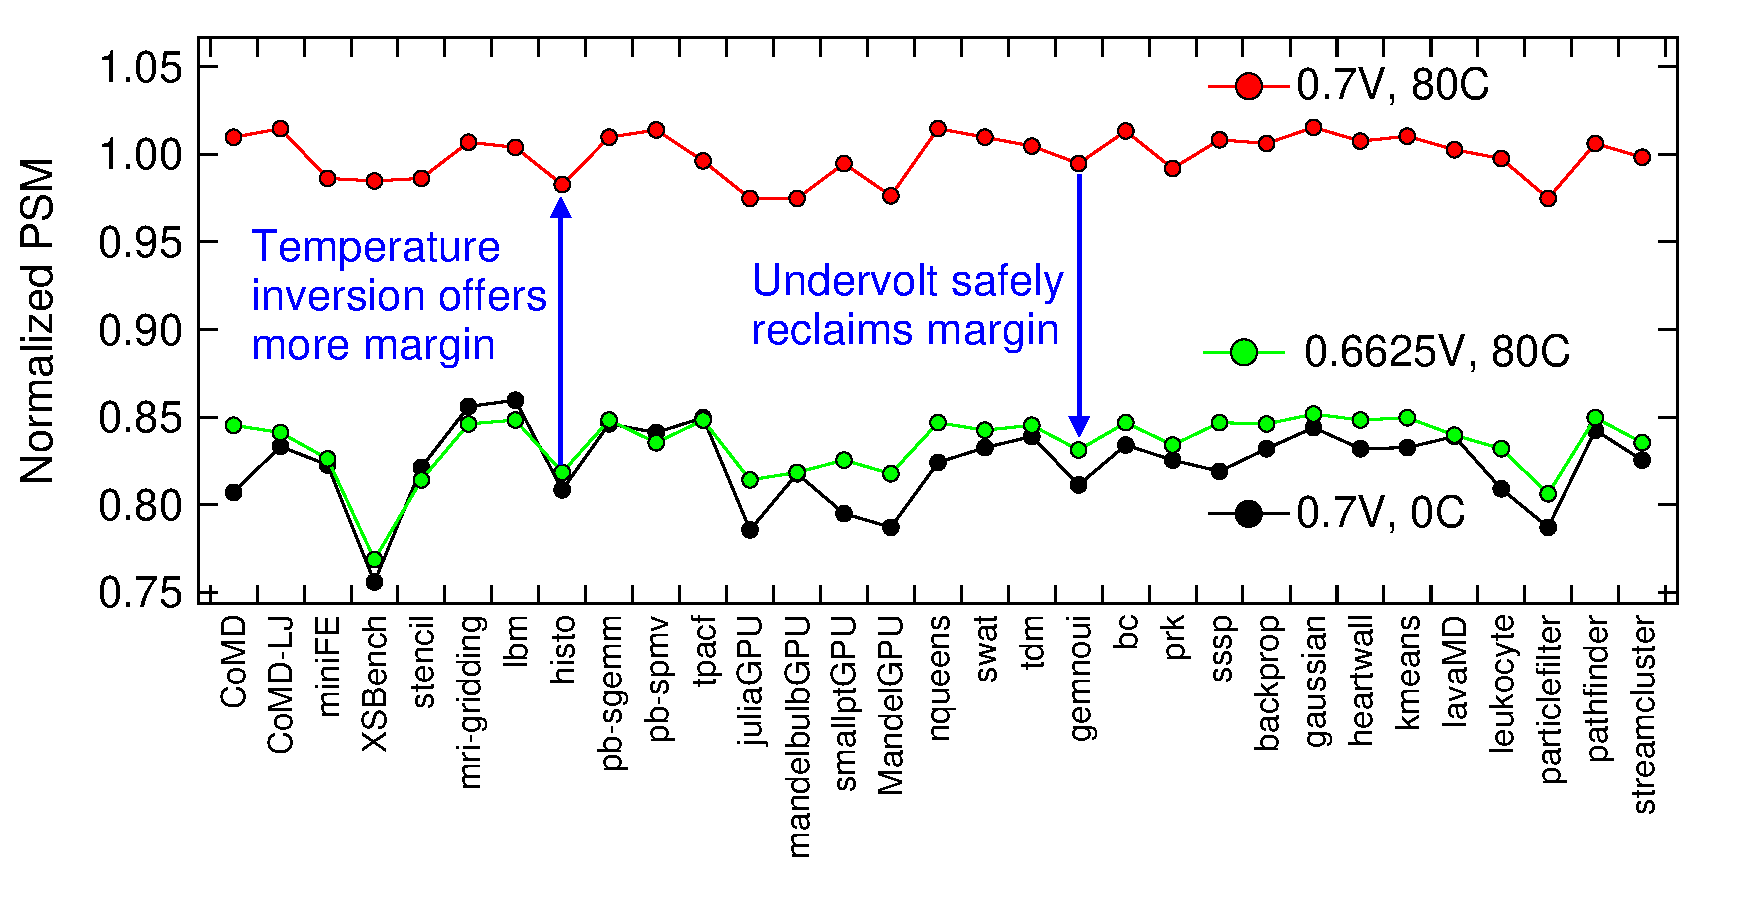
\includegraphics[trim=0 20 30 15,clip,width=\linewidth]{graphs/temperature/validate-uv.pdf}
      \caption{\tistate undervolting decision at 80\C closely tracks the ``golden'' reference runs' timing margin, which is needed for reliability.}
      \label{fig:validate-uv}
\end{figure}

\Fig{fig:validate-uv} verifies \Algo{train-algo}'s \tistate selection at 80\C. At 0.7~V, going from 0\C to 80\C offers more than 15\% extra timing margin. After voltage reduction, the workload timing margins closely track the golden reference with some workloads showing slightly higher margin.

\Fig{fig:validate-uv} proves yet another important point. It shows that the voltage explored using a small set of training workloads can be safely applied to future unknown workloads. The reason that the approach we present works in practice is because the extra margin that arises from temperature inversion is mainly a device property and it is workload-independent.

\subsection{Evaluating Ti-State's Voltage and Power Reduction Effects}
\label{sec:temperature:temperature:table}

\Algo{train-algo} will repeat the same process at different temperatures. Using results similar to~\Fig{fig:train-uv} and \Fig{fig:validate-uv}, our methodology will eventually construct a temperate-voltage pairing table with all the proper \tistates.~\Tab{table:explore-err} shows the measured results on our A10-8700P processor for 20\C, 40\C, 60\C and 80\C. For each temperature, there is one voltage that has the smallest deviation from the ``golden'' reference margin, as highlighted and bolded in the table. These points are selected as the final \tistates for the processor to use.

\begin{table}
\centering
\resizebox{0.75\textwidth}{!}{
	\begin{tabular}{ l | c | c | c | c | c }
    \Xhline{3\arrayrulewidth}
     & {\bf20\C}  & {\bf40\C}  & {\bf60\C}  & {\bf80\C}  & {\bf100\C} \\[1.4ex] \Xhline{3\arrayrulewidth}
    {\bf693.75mV}   &   3.7\% & - & - & - & -  \\
    {\bf687.50mV}   &   \cellcolor{blue!25}{\bf \color{black}2.2\%} &  - & - & - & -  \\
    {\bf681.25mV}   &   8.4\% & \cellcolor{blue!25}{\bf \color{black}2.3\%}  & - & - & -  \\
    {\bf675.00mV}   &   13.9\% & 5.3\% & 4.9\% & - & -  \\
    {\bf668.75mV}   &   - & 9.5\% & \cellcolor{blue!25}{\bf \color{black}2.5\%} &  - & -  \\
    {\bf662.50mV}   &   - & 13.5\% & 6.5\% & \cellcolor{blue!25}{\bf \color{black}1.9\%}  & -  \\
    {\bf656.25mV}   &   - & - & 12.2\% & 5.6\% & 9.9\%  \\
    {\bf650.00mV}   &   - & - & - & 9.3\% & \cellcolor{blue!25}{\bf \color{black}5.1\%}   \\
    \Xhline{3\arrayrulewidth}
  \end{tabular}
}
\vspace{0.2cm}
\caption{PSM error compared to the reference setting for different $<temperature, voltage>$ configurations.}
\label{table:explore-err} 
\end{table}

\tistate table construction would add little overhead to existing silicon test procedures. Per-bin or even per-part characterization is already an industry-standard practice, especially for the high-end server market sector. Therefore, we believe that \tistate table construction is a practical approach.

At runtime, the power management scheme can use temperature sensor data to index into a \tistate table and determine a suitable supply voltage~\cite{sriram2016avfs}. In our work and the restricted scope of this paper, \tistates are constructed for the GPU clock frequency of 300~MHz. In practice, however, the \tistate table can be constructed across different frequencies, and the power management unit can index into the right table by frequency during runtime. 

\begin{figure}[t]
  \centering
  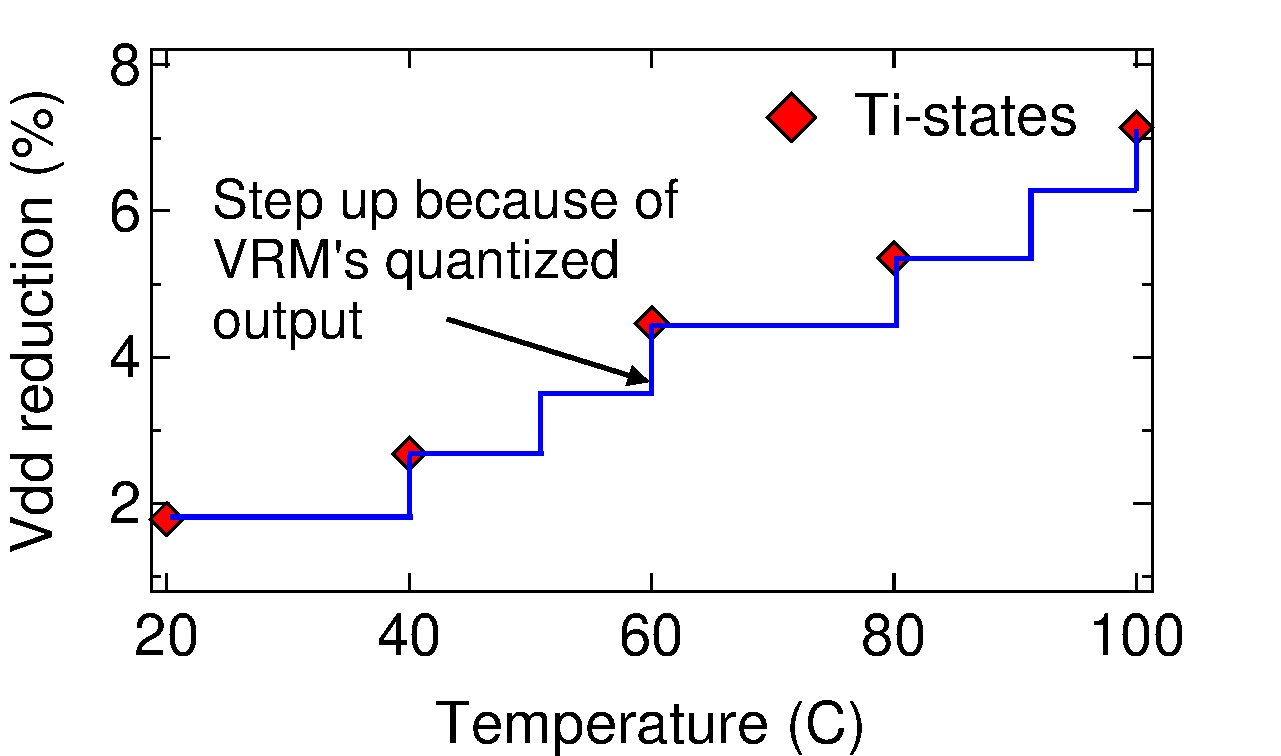
\includegraphics[trim=0 -10 0 0,clip,width=0.7\linewidth]{graphs/temperature/explore-extrapolate.pdf}
  \captionof{figure}{$V_{dd}$ reduction due to \tistates. The line corresponds to the VRM's quantized output values.}
  \label{fig:tistate-show}
\end{figure}

We use a representative subset of all workloads to evaluate \tistate's power reduction at different temperatures. We start with \Fig{fig:tistate-show}, which shows the $V_{dd}$ reduction at various \tistates. One temperature range corresponds to one voltage and this is because of the VRM's quantized output. To make the VRM reduce voltage by one step, the temperature has to be high enough to speed up the circuit beyond the current point. Between 20\C and 40\C, the VRM can reduce $V_{dd}$ by exactly one step, yet from 40\C to 60\C there are two VRM steps in between. The results show that $V_{dd}$ reduction is larger at a higher temperature because the extra timing margin offered by temperature inversion is larger than at a lower temperature. 

\begin{figure}[t]
  \centering
  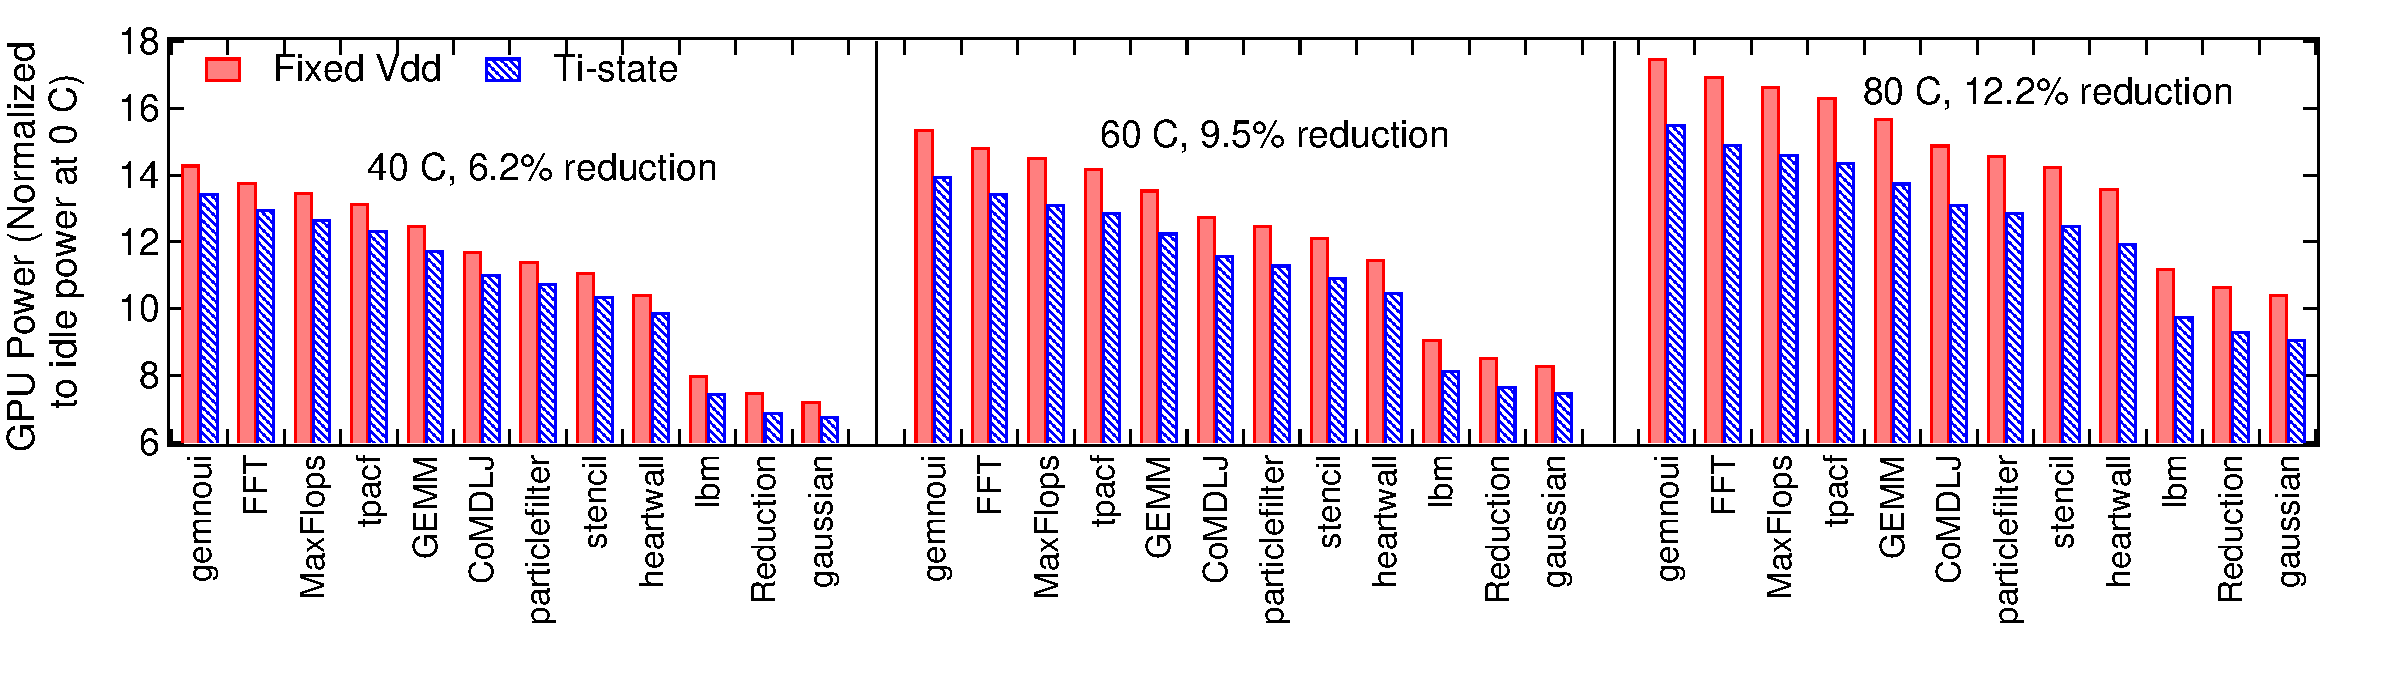
\includegraphics[trim=0 0 0 0,clip,width=\linewidth]{graphs/temperature/evaluate-tistate.pdf}
  \caption{Power saving increases at higher temperatures. We mimic workload temperature by externally controlling die temperature to a 40\C~--~80\C range. \tistate's power reduction is independent of the workload activity. }
  \label{fig:power-save-orig}
\end{figure}

In~\Fig{fig:power-save-orig} we compare the average power savings of the various GPU workloads as a result of the $V_{dd}$ reduction at different temperatures. We set the die temperature manually using our temperature control setup to 40\C, 60\C, and 80\C to mimic the various temperature conditions that the processor typically faces. We manually set the temperature because the GPU on the A10-8700P does not heat up the chip often in the voltage region we study, which limits the temperature range we can use to thoroughly characterize. Therefore, rather than examine the workloads under a ``free run,'' we interject with external temperature control. But on the more high-end and power-hungry server parts, the GPU would hit the higher temperatures we are characterizing.

An added benefit of temperature control is that it facilitates controlled and repeatable experiments. Our choice of temperatures is reasonable because, usually, for a high-end cooling system that has around 0.2\C/W ambient-silicon thermal resistance, a workload consuming 60 W will have a steady state temperature of 40\C. For a less capable 0.5\C/W cooling system the same workload will stabilize around 60\C~\cite{skadron2004temperature,huang2006hotspot,fan2016computational}. So we cover different cooling options.

\Fig{fig:power-save-orig} shows that on average the \tistates can save 6.2\%, 9.5\%, 12.2\% power at 40\C, 60\C and 80\C, respectively. The power saving primarily comes from dynamic power reduction. Leakage power consumption also reduces at lower voltages, but only by a little. At each temperature, the relative power saving does not vary much between different workloads, but this is to be expected because \tistate's voltage reduction is workload independent. Hence, the relative dynamic power saving for each workload should stay the same for each temperature. In practice, different workloads stabilize at different temperatures at runtime, and \tistate will reduce the operating voltage accordingly. When the temperature varies under workload phase changes, a VRM can index into \tistate table in real-time and adjust the supply voltage step by step~\cite{sriram2016avfs}.


\section{Managing Ti-State Processors in Advanced Technology Nodes}
\label{sec:temperature:manage}

In this section, we compare and contrast the benefits of \tistate's power savings on traditional planar bulk CMOS versus the more recent FinFET and FD-SOI process technologies. FinFET is already present in latest processors~\cite{intel22nm,samsung14nm} at the time of this proposal, and both technologies will be more broadly adopted in the coming years~\cite{wu201316nm,natarajan201414nm,lin2014high,liu2014fdsoi}. Because we do not have access to a FinFET or FD-SOI processor to continue our measurement-based study, we scale our measurement results to these technologies. We first explain our scaling approach for FinFET and FD-SOI, then we detail a careful analysis of \tistates in these technologies to show that \tistates may promise an important trade-off between leakage and dynamic power consumption. Finally, we discuss a runtime power management control loop to minimize power consumption by leveraging the optimal temperature(\Sec{sec:runtime}).

\subsection{Scaling to FinFET and FD-SOI}

\begin{table}[t]
\centering
\resizebox{0.75\columnwidth}{!}{
  \begin{tabular}{ c | l | l | l }
      \Xhline{3\arrayrulewidth}
      \pbox{30cm}{Scaling\\setting} & \pbox{20cm}{Leakage\\power} & \pbox{20cm}{Dynamic\\power}  & \pbox{40cm}{Dynamic-leakage\\ Power scale ratio} \\[1.4ex] \Xhline{3\arrayrulewidth}
      {\bf A}   &   0.1 & 1.5 & 15 ~(aggressive) \\
      {\bf B}   &   0.1 & 1 & 10 ~(test-chip \cite{rachala2016amdntc})\\
      {\bf C}   &   0.2 & 1.5 & 7.5 (modest)\\
      {\bf D}   &   0.2 & 1 & 5 ~~(modest)\\
      {\bf E}   &   0.2 & 0.6 & 3 ~~(conservative)\\
      \Xhline{3\arrayrulewidth}
    \end{tabular}
    }
  \caption{FinFET and FD-SOI scaling settings: for completeness, we scale dynamic and leakage power with different factors to cover both aggressive and conservative scenarios.} 
  \label{table:scaling-setting} 
\end{table}

FinFET and FD-SOI technologies can potentially alter high temperature impact total processor power because these technologies' dynamic-to-leakage power ratios are very different from traditional planar bulk CMOS. Here, we set up five reasonable scaling scenarios (ranging from aggressive to conservative leakage reductions) based on lessons from a 14~nm FinFET NTC prototype chip~\cite{rachala2016amdntc} as well as prior report~\cite{pelloux2012planar}. Compared to 28 nm planar bulk CMOS, FinFET can reduce the off-current ($I_{off}$) by more than 10$\times$ under the same supply voltage for all device types, and FD-SOI can achieve even more leakage reduction. We mimic this scenario as setting \marker{B} in~\Tab{table:scaling-setting}. Furthermore, the FinFET test chip runs at 650 MHz at 0.55~V~\cite{rachala2016amdntc}, over 2$\times$ of the 300 MHz frequency we study at 0.7~V. In setting \marker{A}, we scale dynamic power by 1.5 to simulate possible dynamic power changes.

Setting \marker{C}, \marker{D}, and \marker{E} account for possible FinFET threshold voltage engineering by modestly scaling leakage power by 0.2. Setting \marker{C} mimics a performance-centric scenario where lower threshold is utilized for higher frequency. We include setting \marker{E} as a conservative scenario where dynamic power reduces with lower supply voltage. Overall, scaling setting \marker{A} is an aggressive projection for FinFET, but it is a good example of FD-SOI's application scenario. Setting \marker{B} reflects FinFET and FD-SOI's leakage power reduction capability, while settings \marker{C} and \marker{D} represent FinFET's more realistic usage cases. 

Temperature inversion will continue to exist in FinFET and FD-SOI. Prior work concludes FinFET processors will entirely work in temperature inversion range~\cite{lee2014dynamic,cai2015tei}, and its inflection voltage will be around the same as we measure in 28 nm~\cite{lee2014dynamic}. Therefore, we assume the same \tistate's voltage and power reduction capability within these technologies. 

\subsection{\tistate Power Analysis under FinFET and FD-SOI}

\begin{figure}[H]
  \centering 
  \begingroup
  \captionsetup[subfigure]{width=0.5\linewidth}
  \subfloat[Benchmark \benchmark{FFT}]
  {
    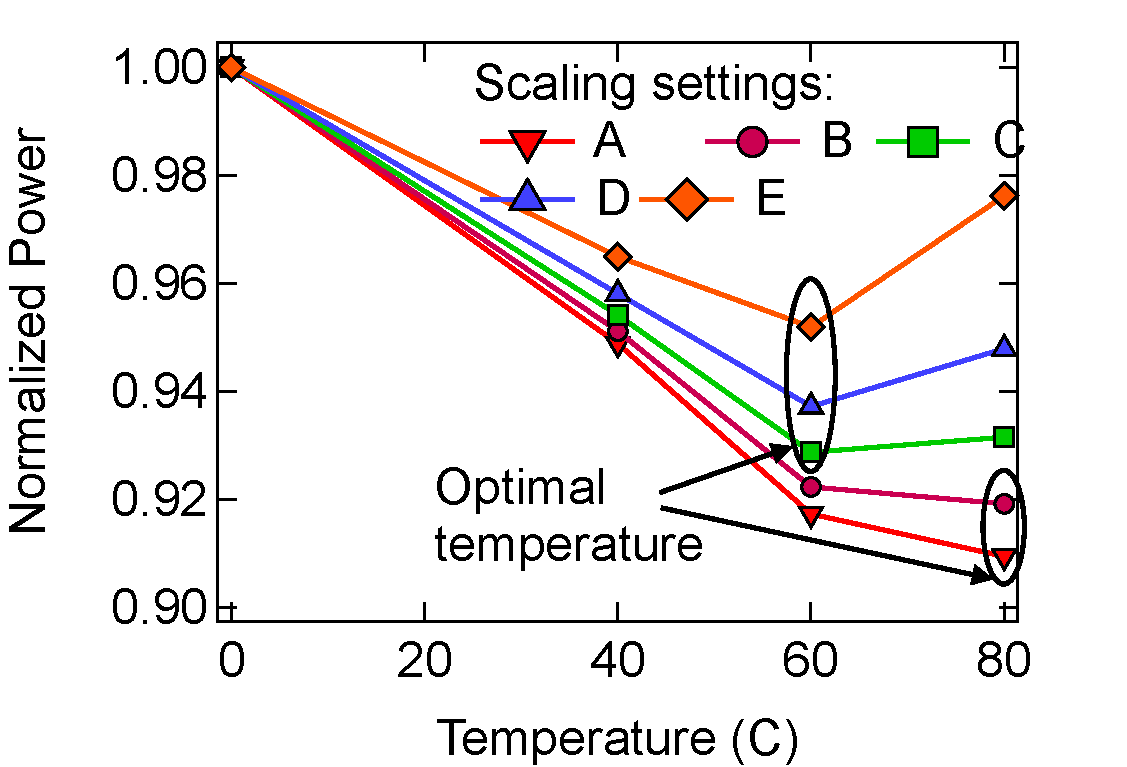
\includegraphics[trim=0 0 40 0,clip,width=0.47\linewidth]{graphs/temperature/FFT-diff-factor.pdf}
    \label{fig:scale-FFT}
  }
  \endgroup
  \hfill
  \begingroup
  \captionsetup[subfigure]{width=0.\linewidth}
  \subfloat[Benchmark \benchmark{particlefilter}] 
  {
    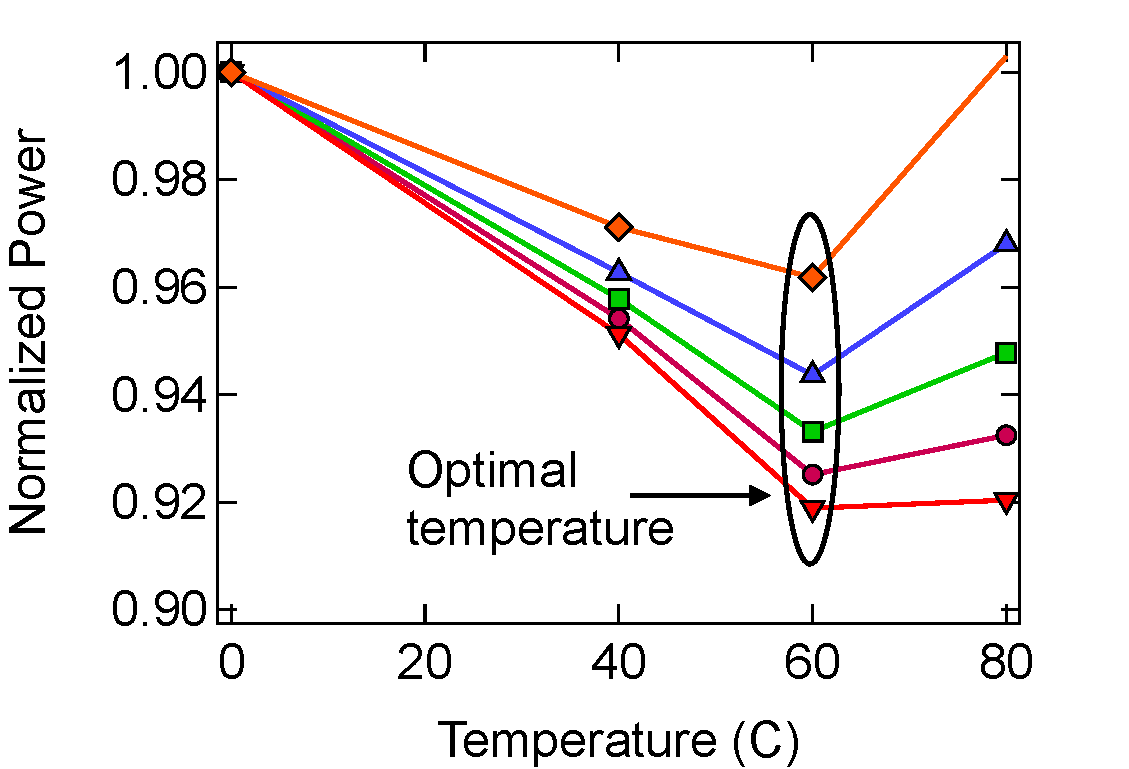
\includegraphics[trim=0 0 40 0,clip,width=0.47\linewidth]{graphs/temperature/particlefilter-diff-factor.pdf}
    \label{fig:scale-particlefilter}
  }
  \endgroup

  \begingroup
  \captionsetup[subfigure]{width=0.3\linewidth}
  \subfloat[Benchmark \benchmark{Reduction}] 
  {
    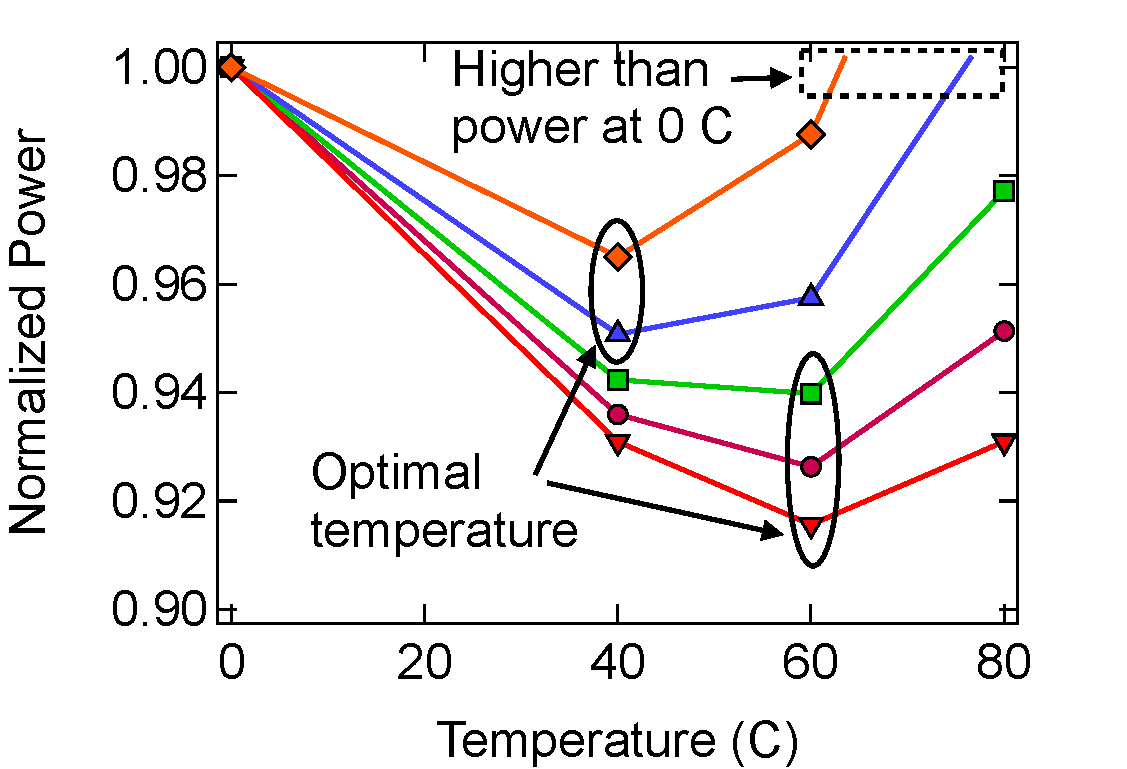
\includegraphics[trim=0 0 40 0,clip,width=0.47\linewidth]{graphs/temperature/Reduction-diff-factor.pdf}
    \label{fig:scale-Reduction}
  }
  \endgroup
  \caption{Power versus temperature under different scaling factors for different workloads. In FinFET and FD-SOI, \tistate makes GPU power smaller at high temperature. The optimal temperature is different for the workloads and the different scaling settings, and this is because the ratio of static to dynamic power across the workloads varies.}
  \label{fig:scale-analysis}
\end{figure}

Thus far, we have shown the total power savings from \tistate as a result of voltage reduction under a particular temperature level, which is set by the thermal headset. However, high temperature still increases leakage power exponentially, especially in planar bulk CMOS technology, which is against the dynamic power savings from \tistate with voltage reduction at high temperature. The overall effect of these two opposite factors in bulk CMOS is that processors still favor lower temperature for power reduction. 

In FinFET and FD-SOI, the scenario above will fundamentally change. FinFET and FD-SOI have much less leakage power, therefor the leakage power increase has a smaller effect on overall processor power under higher temperature. The opposite side is the more salient dynamic power improvement caused by \tistate's voltage reduction. These two opposite trends form a trade-off: an optimal temperature may exist where \tistate's dynamic power reduction balances leakage power increase at higher temperatures and the overall processor power is minimized. Carefully evaluating this trade-off is crucial for \tistate to be practical in runtime processor temperature and power management control. 

We examine \tistate's power benefits on FinFET and FD-SOI for three different types of workloads that are representative of different typical dynamic-to-leakage power ratios. The workloads include \benchmark{FFT}, \benchmark{particlefilter} and \benchmark{Reduction}, going from high to low dynamic power consumption. \Fig{fig:scale-analysis} shows \tistate's GPU power under different scaling settings. Power is normalized to 0\C to show how power scales as temperature increases. 

\Fig{fig:scale-FFT} shows that when the dynamic power is more dominant in settings \marker{A} and \marker{B} then \benchmark{FFT} prefers to stay at 80\C. Under more conservative settings where leakage power is higher, the temperature sweet spot drops to 60\C. In these scaling settings, FinFET's leakage power increase beyond 60\C is more than \tistate's dynamic power reduction.

For medium dynamic power, \Fig{fig:scale-particlefilter} shows that \benchmark{particlefilter}'s temperature sweet spot is around 60\C for the scaling ratios. \benchmark{Particlefilter}'s dynamic power is not high enough to make \tistate's power saving override leakage power at 80\C. 

In contrast to \benchmark{FFT} and \benchmark{particlefilter}, the workload \benchmark{Reduction} does not consume much dynamic power. \Fig{fig:scale-Reduction} shows that it prefers to stay at a lower temperature to minimize leakage power. Its dynamic power occupies a smaller portion of total power, therefore \tistate's power reduction has a lesser effect. In the optimistic scaling settings \marker{A} and \marker{B}, \benchmark{Reduction}'s sweet spot temperature is 60\C, whereas in conservative settings \marker{D} and \marker{E}, the optimal temperature is at 40\C to avoid the exponential leakage power at a higher temperature. 

In general, \Fig{fig:scale-analysis} shows that when leakage power is less prominent (i.e., leakage scaling is more aggressive in~\Tab{table:scaling-setting}), \tistates have higher power saving and the optimal temperature is also higher. With smaller leakage, dynamic power occupies a larger portion of the total power, which is when \tistate's improvement has a bigger power saving impact. In the extreme assumption where leakage power is completely agnostic of temperature, \tistate would prefer to operate at the highest allowed temperature to maximize the magnitude of voltage reduction from temperature inversion.

We also find when the optimal temperature is higher, the corresponding optimal power tends to be lower as well.  \tistate's power saving capability increases with higher temperature. When a workload has a larger share of dynamic power and prefers to run under a higher temperature, \tistate's higher power saving manifests as total power improvement.

Another observation that we can make from~\Fig{fig:scale-analysis} is that high-power workloads typically have higher temperature sweet spots. For such workloads, the dynamic power is more dominant than the leakage power. Therefore, in such scenarios, for a given temperature, the percentage of dynamic power saving from \tistate contributes more to the bottom-line.

\subsection{Runtime Temperature Control}
\label{sec:runtime}

\begin{figure*}[t!]
\centering
    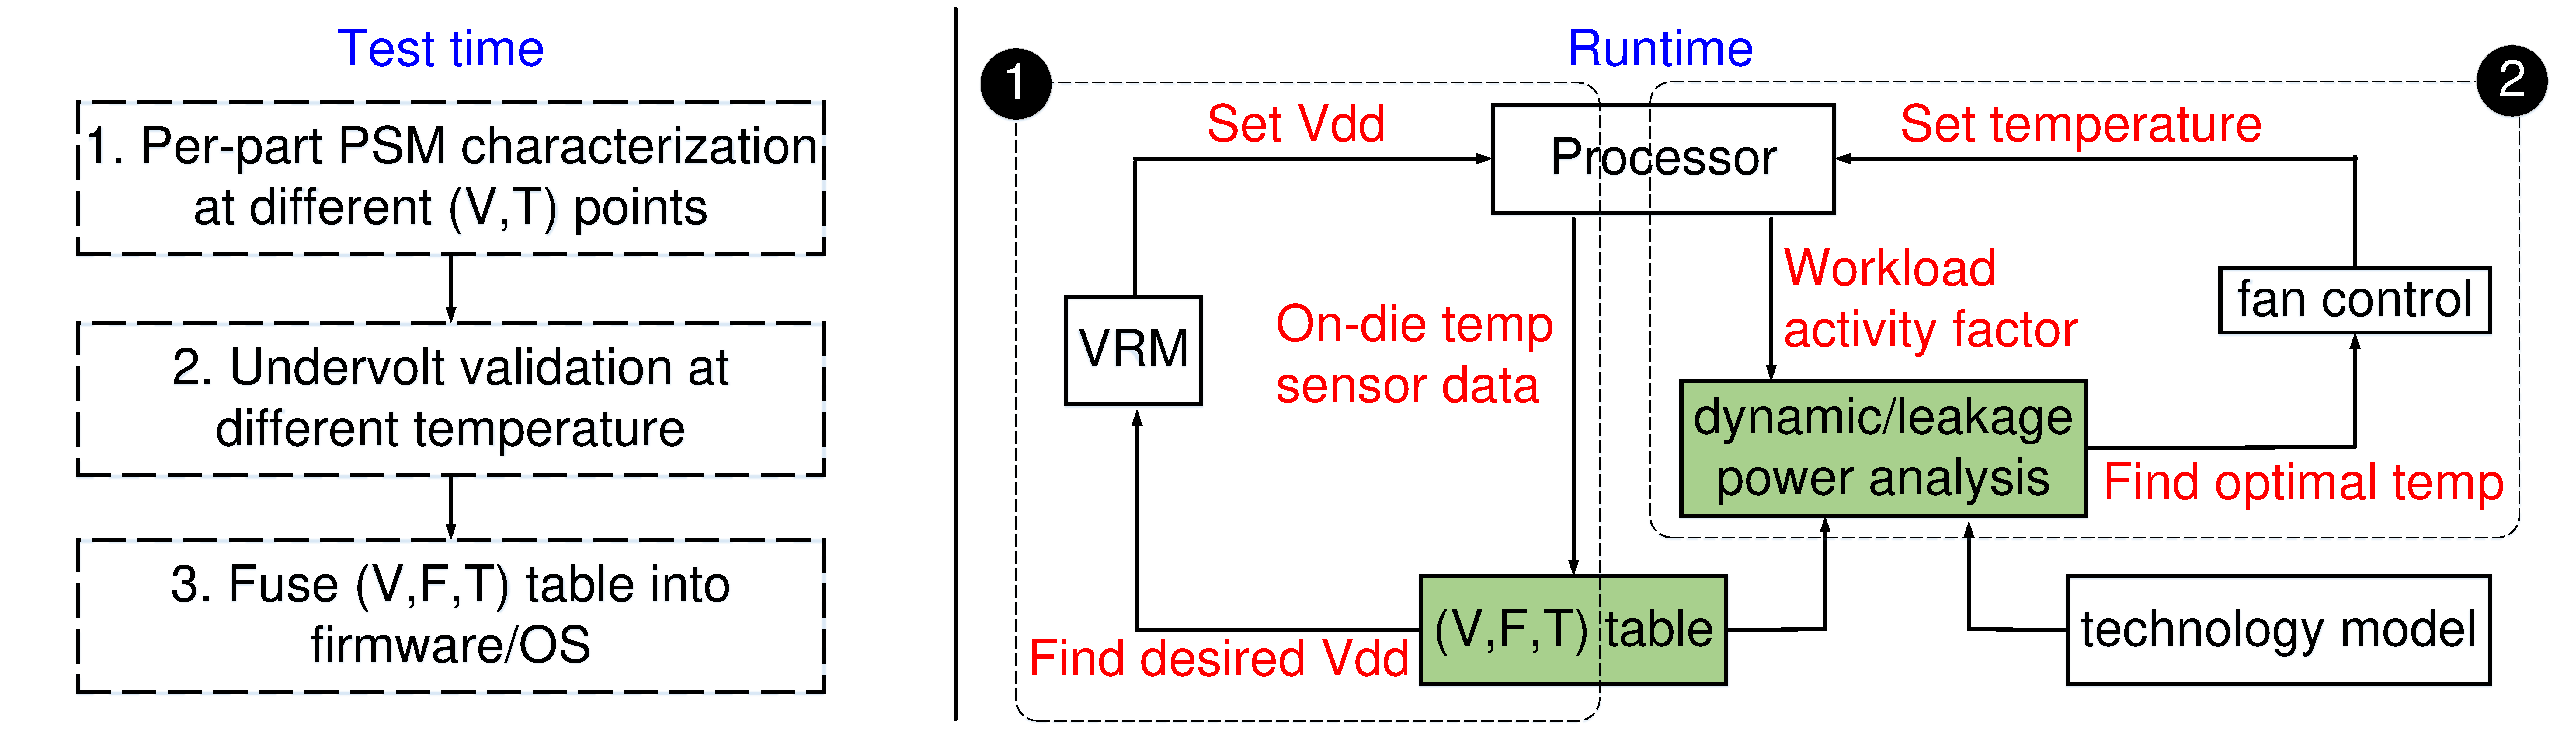
\includegraphics[trim=0 0 0 0,clip,width=.96\linewidth]{graphs/temperature/runtime-mechanism_v3.pdf}
    \caption{\tistate temperature and voltage control: two loops work in synergy to minimize power. Loop~1 is a fast control loop that uses \tistate table to keep adjusting voltage in response to silicon temperature variation. Loop~2 is a slow control loop that sets the optimal temperature based on workload steady-state dynamic power profile.}
    \label{fig:runtime}
    \vspace*{-.1in}
\end{figure*}

We notice that different temperature sweet spots under all workloads and scaling scenarios are essentially a result of processor's dynamic-to-leakage power ratio. To leverage this fact, we propose a set of temperature and voltage control algorithms in~\Fig{fig:runtime} to steer future FinFET and FD-SOI processors for maximum power efficiency. The solution consists of two stages: test-time and runtime.

At test time, the methodology described in~\Algo{train-algo} establishes \tistate's temperature-voltage tables.  The process starts with characterizing the circuit speed behavior with on-chip timing sensors like the PSM, which are subsequently verified by workload timing margin measurements as we described earlier. The final temperature-voltage table can be fused into firmware for runtime lookup. For each chip, we envision less than 40 entries to be added in total. Constructing such tables is already in practice~\cite{sriram2016avfs}. It only extends the existing test flow by a few steps, and adds minimal overhead.

At runtime, two loops work in synergy. Loop 1 is a fast loop that addresses quick yet small temperature variations from workload phase changes. It measures silicon temperature and index into \tistate table in real time to get and set the desired voltage, similar to a typical DVFS table lookup. We envision this loop to occur at millisecond-level granularity, as in with other systems~\cite{lefurgy2011active}. Loop 2 is a slow control loop that monitors the workload's average activity factor over a longer time period to estimate its dynamic-to-leakage power ratio. This ratio is used to find the optimal temperature in~\Fig{fig:scale-analysis}, and hence discovers the \tistate's optimal long-term average voltage.

We envision that loop 2 will target the average power savings over a relatively long time (seconds or longer). This is because runtime temperature control by adjusting the cooling system is a relatively slow process. Many of today's workload have steady state behavior suitable for this behavior, such as scientific and deep learning applications, as well as web service workloads that have diurnal patterns~\cite{lo2014towards}. Thus, it is feasible to enable power saving in this scenario.

\section{Related Work}
\label{sec:temperature:related}

Temperature inversion has been reported for CMOS devices long before~\cite{park1995reversal,bellaouar1998supply,dasdan2006handling,wolpert2012temperature}. These works address the reason for this phenomenon, largely at the device level. Recent works study temperature inversion in FinFETs~\cite{lee2014dynamic,cai2015tei}. Our work, however, is the first to systematically measure and characterize temperature inversion under 28 nm process and discuss its implications to the architecture and its power management. 

Adaptive voltage setting for temperature variation has been recently proposed~\cite{sriram2016avfs}. \tistates work in a similar way to the lookup table that the authors propose. However, our work focuses on the temperature's effect in the inversion region and provides an in-depth analysis, while the solution in~\cite{sriram2016avfs} mixes process and temperature variation together. Moreover, prior work does not address the implications of temperature control in future technologies, as we do with our FinFET analysis.

Active timing guardband management using on-chip sensors has been recently proposed~\cite{lefurgy2011active,zu2015adaptive}. These prior works focus mostly on transient $di/dt$ droop and its effect on the timing margin. In contrast, we use PSMs to characterize temperature inversion and its effect on the timing margin. We also study temperature inversion's effect in an integrated manner with $di/dt$ droop and discuss the relationship between the two.

Many papers have addressed architecture-level temperature management~\cite{skadron2004temperature,huang2006hotspot,fan2016computational,raghavan2012computational}. These works try to avoid excess high temperature. But we demonstrate experimentally how temperature inversion can make high temperature a friendly environment for runtime power management.

